% =====================================================================
%  Chapter 11: Triple and Higher-Dimensional Integrals
% =====================================================================

\chapter{Triple and Higher-Dimensional Integrals}
\label{ch:11}

Chapter \ref{ch:10} ended with a double integral spread over a thin region: a floor, a
map, a plate, a lamina.  The tiny pieces were small rectangles, and each one carried a
small contribution
\[
    f(x,y)\,\Delta A.
\]

Many quantities do not live on a thin sheet.  Air fills a room.  Density fills a solid ball.
Charge may be spread throughout a three-dimensional object.  The same adding idea
still works, but the small pieces are no longer small rectangles.  They are small boxes.

\section{Triple integrals}
\label{sec:11.1}

A double integral adds over area.  A triple integral adds over volume.

That one sentence is almost the whole idea.  But it is worth seeing it first in the
plainest possible place: a rectangular box.

\subsection{Volume as a triple integral}

Imagine a storage room whose dimensions are
\[
    4\text{ m}\times 3\text{ m}\times 2\text{ m}.
\]
Its volume is
\[
    4\cdot 3\cdot 2=24\text{ m}^3.
\]
Now suppose we forget that formula and rebuild the answer by adding small boxes.

Cut the room into unit cubes.  Each cube has volume
\[
    1\text{ m}^3.
\]
There are
\[
    4\cdot3\cdot2=24
\]
of them, so the total volume is
\[
    24\cdot1=24.
\]

If the cubes were smaller, the idea would be the same.  A small box with side lengths
\[
    \Delta x,\qquad \Delta y,\qquad \Delta z
\]
has volume
\[
    \Delta V=\Delta x\,\Delta y\,\Delta z.
\]
Adding all those small volumes gives the volume of the room:
\[
    \sum \Delta V.
\]
In integral notation,
\[
\boxed{
    \operatorname{Volume}(E)=\iiint_E 1\,dV.
}
\]
This says: add the constant value \(1\) throughout the solid \(E\).

\begin{figure}[h]
\centering
\begin{tikzpicture}
    \begin{axis}[
        view={35}{25},
        width=11cm, height=8.5cm,
        axis lines=none,
        clip=false,
        xmin=0, xmax=5,
        ymin=0, ymax=4,
        zmin=0, zmax=3
    ]
        % 1. 3D Grid lines (BEHIND the red box)
        % x-lines
        \foreach \y in {0,...,2} {
            \foreach \z in {0,1} {
                \edef\temp{
                    \noexpand\draw[gray!70, thin] (0,\y,\z) -- (3,\y,\z);
                }\temp
            }
        }
        % y-lines
        \foreach \x in {0,...,3} {
            \foreach \z in {0,1} {
                \edef\temp{
                    \noexpand\draw[gray!70, thin] (\x,0,\z) -- (\x,2,\z);
                }\temp
            }
        }
        % z-lines
        \foreach \x in {0,...,3} {
            \foreach \y in {0,...,2} {
                \edef\temp{
                    \noexpand\draw[gray!70, thin] (\x,\y,0) -- (\x,\y,1);
                }\temp
            }
        }

        % 2. Highlighted Red Box (Delta V) deep inside the grid
        % Fill the 6 faces (ordered back-to-front for proper 3D shading)
        % Bottom
        \fill[red!40, opacity=0.5] (2,1,0) -- (3,1,0) -- (3,2,0) -- (2,2,0) -- cycle;
        % Back-Left (x=2)
        \fill[red!50, opacity=0.5] (2,1,0) -- (2,2,0) -- (2,2,1) -- (2,1,1) -- cycle;
        % Back-Right (y=1)
        \fill[red!50, opacity=0.5] (2,1,0) -- (3,1,0) -- (3,1,1) -- (2,1,1) -- cycle;
        % Top
        \fill[red!60, opacity=0.5] (2,1,1) -- (3,1,1) -- (3,2,1) -- (2,2,1) -- cycle;
        % Front-Left (x=3)
        \fill[red!70, opacity=0.5] (3,1,0) -- (3,2,0) -- (3,2,1) -- (3,1,1) -- cycle;
        % Front-Right (y=2)
        \fill[red!60, opacity=0.5] (2,2,0) -- (3,2,0) -- (3,2,1) -- (2,2,1) -- cycle;

        % Draw the 12 edges with a dashed pattern
        \draw[red!80!black, thick, dashed] 
            (2,1,0) -- (3,1,0) -- (3,2,0) -- (2,2,0) -- cycle % bottom
            (2,1,1) -- (3,1,1) -- (3,2,1) -- (2,2,1) -- cycle % top
            (2,1,0) -- (2,1,1) % vertical 1
            (3,1,0) -- (3,1,1) % vertical 2
            (3,2,0) -- (3,2,1) % vertical 3
            (2,2,0) -- (2,2,1); % vertical 4

        % 3. 3D Grid lines (IN FRONT OF the red box)
        % x-lines
        \foreach \y in {0,...,2} {
            \foreach \z in {0,1} {
                \edef\temp{
                    \noexpand\draw[gray!70, thin] (3,\y,\z) -- (4,\y,\z);
                }\temp
            }
        }
        \foreach \z in {0,...,2} {
            \edef\temp{
                \noexpand\draw[gray!70, thin] (0,3,\z) -- (4,3,\z);
            }\temp
        }
        \foreach \y in {0,...,2} {
            \edef\temp{
                \noexpand\draw[gray!70, thin] (0,\y,2) -- (4,\y,2);
            }\temp
        }

        % y-lines
        \foreach \x in {0,...,3} {
            \foreach \z in {0,1} {
                \edef\temp{
                    \noexpand\draw[gray!70, thin] (\x,2,\z) -- (\x,3,\z);
                }\temp
            }
        }
        \foreach \z in {0,...,2} {
            \edef\temp{
                \noexpand\draw[gray!70, thin] (4,0,\z) -- (4,3,\z);
            }\temp
        }
        \foreach \x in {0,...,3} {
            \edef\temp{
                \noexpand\draw[gray!70, thin] (\x,0,2) -- (\x,3,2);
            }\temp
        }

        % z-lines
        \foreach \x in {0,...,3} {
            \foreach \y in {0,...,2} {
                \edef\temp{
                    \noexpand\draw[gray!70, thin] (\x,\y,1) -- (\x,\y,2);
                }\temp
            }
        }
        \foreach \y in {0,...,3} {
            \edef\temp{
                \noexpand\draw[gray!70, thin] (4,\y,0) -- (4,\y,2);
            }\temp
        }
        \foreach \x in {0,...,3} {
            \edef\temp{
                \noexpand\draw[gray!70, thin] (\x,3,0) -- (\x,3,2);
            }\temp
        }

        % 4. Semi-transparent exterior glass faces
        % Top glass face (z=2)
        \foreach \x in {0,...,3} {
            \foreach \y in {0,...,2} {
                \pgfmathsetmacro{\xp}{\x+1}
                \pgfmathsetmacro{\yp}{\y+1}
                \edef\temp{
                    \noexpand\filldraw[fill=cyan!15, fill opacity=0.4, draw=cyan!70!black, thin]
                        (\x,\y,2) -- (\xp,\y,2) -- (\xp,\yp,2) -- (\x,\yp,2) -- cycle;
                }\temp
            }
        }
        % Front-Left glass face (x=4)
        \foreach \y in {0,...,2} {
            \foreach \z in {0,1} {
                \pgfmathsetmacro{\yp}{\y+1}
                \pgfmathsetmacro{\zp}{\z+1}
                \edef\temp{
                    \noexpand\filldraw[fill=cyan!30, fill opacity=0.4, draw=cyan!70!black, thin]
                        (4,\y,\z) -- (4,\yp,\z) -- (4,\yp,\zp) -- (4,\y,\zp) -- cycle;
                }\temp
            }
        }
        % Front-Right glass face (y=3)
        \foreach \x in {0,...,3} {
            \foreach \z in {0,1} {
                \pgfmathsetmacro{\xp}{\x+1}
                \pgfmathsetmacro{\zp}{\z+1}
                \edef\temp{
                    \noexpand\filldraw[fill=cyan!45, fill opacity=0.4, draw=cyan!70!black, thin]
                        (\x,3,\z) -- (\xp,3,\z) -- (\xp,3,\zp) -- (\x,3,\zp) -- cycle;
                }\temp
            }
        }

        % 5. Labels for dimensions (attached to the front-most edges)
        \node[anchor=south east, font=\small] at (2.7,-0.9,0) {\(4\text{ m}\)};
        \node[anchor=north west, font=\small] at (4,1.5,0) {\(3\text{ m}\)};
        \node[anchor=west, font=\small] at (4,3,1) {\(2\text{ m}\)};

        % 6. Pointer for the small volume
        \draw[<-, thick, red!80!black] (2.5, 1.5, 1.0) -- (4.8, 1.5, 2.5) 
            node[above right, text=black] {small box \(\Delta V\)};

    \end{axis}
    
    % Main caption node correctly anchored below the 3D axis
    \node at (current bounding box.south) [below=2ex] {a box built from smaller boxes};
\end{tikzpicture}
\caption{A triple integral begins by adding tiny volume pieces.}
\end{figure}

Now put a quantity inside the room.  Suppose the density of a gas is
\[
    \rho(x,y,z)=1+\frac z2
\]
kilograms per cubic meter.  The density is larger near the ceiling.

A small box near \((x,y,z)\) has mass approximately
\[
    \rho(x,y,z)\,\Delta V.
\]
Adding all small masses gives the total mass:
\[
\boxed{
    M=\iiint_E \rho(x,y,z)\,dV.
}
\]

For our room,
\[
    E=[0,4]\times[0,3]\times[0,2].
\]
The mass is
\[
\begin{aligned}
M
&=
\int_0^4\int_0^3\int_0^2
\left(1+\frac z2\right)\,dz\,dy\,dx\\
&=
\int_0^4\int_0^3
\left[
z+\frac{z^2}{4}
\right]_{0}^{2}
\,dy\,dx\\
&=
\int_0^4\int_0^3 3\,dy\,dx\\
&=
\int_0^4 9\,dx\\
&=
36.
\end{aligned}
\]
So the gas has total mass
\[
\boxed{
    36\text{ kg}.
}
\]

The calculation did exactly what the story said.  It added density times small volume
throughout the room.

\begin{definition}[Triple integral, first meaning]
Let \(E\) be a solid region in space.  If sums of the form
\[
    \sum f(x_i^*,y_i^*,z_i^*)\,\Delta V_i
\]
approach one number as the small volume pieces shrink, independent of the sample
points, then that number is called the \emph{triple integral} of \(f\) over \(E\), written
\[
\boxed{
    \iiint_E f(x,y,z)\,dV.
}
\]
\end{definition}

The symbol \(dV\) means a tiny positive volume piece.

There is also an oriented version.  In Chapter \ref{ch:2}, the form
\[
    dx\wedge dy\wedge dz
\]
measured signed volume.  For a small box whose edges point first in the positive
\(x\)-direction, then the positive \(y\)-direction, then the positive \(z\)-direction,
\[
    dx\wedge dy\wedge dz
\]
gives
\[
    \Delta x\,\Delta y\,\Delta z.
\]
So the oriented version of a triple integral is
\[
\boxed{
    \iiint_E f(x,y,z)\,dx\wedge dy\wedge dz.
}
\]
For volume, mass, probability, and energy, we usually write \(dV\), because those
quantities use positive volume.  The wedge notation remembers orientation, and that
memory will matter when surfaces acquire a chosen side.

\subsection{Integrals over boxes}

A rectangular box has the form
\[
    B=[a,b]\times[c,d]\times[e,f].
\]
That means
\[
    a\le x\le b,\qquad c\le y\le d,\qquad e\le z\le f.
\]

To build a Riemann sum, cut the three coordinate intervals into pieces.  A typical
small box has side lengths
\[
    \Delta x_i,\qquad \Delta y_j,\qquad \Delta z_k,
\]
so its volume is
\[
    \Delta V_{ijk}
    =
    \Delta x_i\,\Delta y_j\,\Delta z_k.
\]
Choose a sample point
\[
    (x_{ijk}^*,y_{ijk}^*,z_{ijk}^*)
\]
inside that small box.  The Riemann sum is
\[
\boxed{
    \sum_i\sum_j\sum_k
    f(x_{ijk}^*,y_{ijk}^*,z_{ijk}^*)\,
    \Delta V_{ijk}.
}
\]

The table below gives the common meanings.

\[
\begin{array}{c|c|c}
\text{Function} & \text{Units of } f & \text{Meaning of } \displaystyle\iiint_E f\,dV \\ \hline
f(x,y,z)=1 & 1 & \text{volume of }E\\[1mm]
\rho(x,y,z)=\text{density} & \text{kg/m}^3 & \text{mass}\\[1mm]
q(x,y,z)=\text{charge density} & \text{C/m}^3 & \text{total charge}\\[1mm]
u(x,y,z)=\text{energy density} & \text{J/m}^3 & \text{total energy}\\[1mm]
p(x,y,z)=\text{probability density} & 1/\text{volume} & \text{probability}
\end{array}
\]

\begin{example}[Total charge in a box]
A solid block occupies
\[
    B=[0,2]\times[0,1]\times[0,3].
\]
Its charge density is
\[
    q(x,y,z)=6+x+2y+3z.
\]
The total charge is
\[
    Q=\iiint_B q(x,y,z)\,dV.
\]
Using the order \(dz\,dy\,dx\),
\[
\begin{aligned}
Q
&=
\int_0^2\int_0^1\int_0^3
(6+x+2y+3z)\,dz\,dy\,dx.
\end{aligned}
\]
First integrate with respect to \(z\):
\[
\begin{aligned}
\int_0^3(6+x+2y+3z)\,dz
&=
\left[(6+x+2y)z+\frac32z^2\right]_0^3\\
&=
3(6+x+2y)+\frac{27}{2}\\
&=
\frac{63}{2}+3x+6y.
\end{aligned}
\]
Then integrate with respect to \(y\):
\[
\begin{aligned}
\int_0^1
\left(
\frac{63}{2}+3x+6y
\right)\,dy
&=
\frac{63}{2}+3x+3\\
&=
\frac{69}{2}+3x.
\end{aligned}
\]
Finally,
\[
\begin{aligned}
Q
&=
\int_0^2
\left(
\frac{69}{2}+3x
\right)\,dx\\
&=
69+6\\
&=
75.
\end{aligned}
\]
So
\[
\boxed{
    Q=75.
}
\]
\end{example}

The order \(dz\,dy\,dx\) tells us to integrate in \(z\) first, then \(y\), then \(x\).
It is an instruction for computation.

The oriented volume form
\[
    dx\wedge dy\wedge dz
\]
is different.  It remembers the orientation of ordered directions:
\[
    dx\wedge dy\wedge dz
    =
    -dy\wedge dx\wedge dz.
\]
For ordinary triple integrals with \(dV\), the order of calculation does not change the
sign.  The bounds and the differentials only tell us how to do the arithmetic.

\subsection{Iterated triple integrals}

The expression
\[
    \int_a^b\int_c^d\int_e^f f(x,y,z)\,dz\,dy\,dx
\]
means
\[
    \int_a^b
    \left(
        \int_c^d
        \left(
            \int_e^f f(x,y,z)\,dz
        \right)
        dy
    \right)
    dx.
\]
In the innermost integral, \(x\) and \(y\) are held constant while \(z\) changes.  After
that, \(x\) is held constant while \(y\) changes.  The outermost integral finally adds the
results over \(x\).

\begin{definition}[Iterated triple integral over a box]
For a box
\[
    B=[a,b]\times[c,d]\times[e,f],
\]
the iterated integral
\[
\boxed{
    \int_a^b\int_c^d\int_e^f f(x,y,z)\,dz\,dy\,dx
}
\]
means that \(z\) is integrated first, then \(y\), then \(x\).

Other orders are read the same way.  The differential closest to the integrand is the
first variable integrated.
\end{definition}

There are six possible orders:
\[
\begin{array}{ccc}
dz\,dy\,dx, & dz\,dx\,dy, & dy\,dz\,dx,\\[1mm]
dy\,dx\,dz, & dx\,dz\,dy, & dx\,dy\,dz.
\end{array}
\]
For boxes and well-behaved functions, all six orders give the same total.

\begin{theorem}[Fubini's theorem for boxes]
Let
\[
    B=[a,b]\times[c,d]\times[e,f],
\]
and suppose \(f\) is continuous on \(B\).  Then
\[
\boxed{
    \iiint_B f(x,y,z)\,dV
}
\]
can be computed by any of the six iterated integrals.  For example,
\[
\boxed{
\iiint_B f\,dV
=
\int_a^b\int_c^d\int_e^f f(x,y,z)\,dz\,dy\,dx
=
\int_e^f\int_c^d\int_a^b f(x,y,z)\,dx\,dy\,dz.
}
\]
\end{theorem}

Continuity is a safe condition.  It guarantees that the volume sums settle down and that
slicing in any coordinate order gives the same total.  It is stronger than necessary.  A
density with a jump across a plane can still be integrable.

\begin{example}[A jump can still be integrated]
On the box
\[
    B=[0,1]\times[0,1]\times[0,2],
\]
define
\[
    f(x,y,z)=
    \begin{cases}
    2, & 0\le z<1,\\
    5, & 1\le z\le2.
    \end{cases}
\]
The function jumps across the plane \(z=1\), so it is not continuous.  But the integral
is still easy.  The lower half of the box contributes
\[
    2\cdot 1=2,
\]
and the upper half contributes
\[
    5\cdot 1=5.
\]
Thus
\[
\boxed{
    \iiint_B f\,dV=7.
}
\]
So continuity is not the point by itself.  The point is that the adding process must have
a well-defined limit.
\end{example}

Here is what breaks when the adding process does not settle.

\begin{example}[Why integrability is needed]
Define a function on
\[
    B=[0,1]\times[0,1]\times[0,1]
\]
by
\[
    q(x,y,z)=
    \begin{cases}
    1, & x\text{ is rational},\\
    0, & x\text{ is irrational}.
    \end{cases}
\]
Every small box contains points with rational \(x\)-coordinate and points with irrational
\(x\)-coordinate.  So on every small box, the largest possible value of \(q\) is \(1\), and
the smallest possible value is \(0\).

The upper sums always give the full volume:
\[
    1.
\]
The lower sums always give
\[
    0.
\]
They cannot approach the same number.  Therefore
\[
    \iiint_B q\,dV
\]
does not exist as a Riemann integral.

This example is not a model for a physical density.  It is a warning label for the
theorem: before changing orders, there must be an integral to change.
\end{example}

\begin{proof}[Idea of Fubini's theorem for boxes]
A triple integral over a box adds small contributions
\[
    f(x,y,z)\,\Delta x\,\Delta y\,\Delta z.
\]
An iterated integral groups those same small contributions into slices.

For example, if we integrate in \(z\) first, we add the thin vertical column above a fixed
point \((x,y)\).  Then we add those columns over \(y\), and finally over \(x\).

If we integrate in \(x\) first, we group the same small boxes into slabs pointing in a
different direction.  The small contributions are the same; only the grouping changes.
For continuous \(f\), the limits of these grouped sums agree.
\end{proof}

\subsection{Order of integration in space}

For a rectangular box, changing the order is mostly a matter of taste.  The limits stay
constant.

Return to the density
\[
    \rho(x,y,z)=1+\frac z2
\]
on
\[
    B=[0,4]\times[0,3]\times[0,2].
\]
The order \(dz\,dy\,dx\) gave
\[
    \int_0^4\int_0^3\int_0^2
    \left(1+\frac z2\right)\,dz\,dy\,dx.
\]
Since the density depends only on \(z\), it may feel more natural to leave \(z\) for last:
\[
\begin{aligned}
M
&=
\int_0^2\int_0^3\int_0^4
\left(1+\frac z2\right)\,dx\,dy\,dz\\
&=
\int_0^2\int_0^3
4\left(1+\frac z2\right)\,dy\,dz\\
&=
\int_0^2
12\left(1+\frac z2\right)\,dz\\
&=
12\left[z+\frac{z^2}{4}\right]_0^2\\
&=
36.
\end{aligned}
\]
The same mass appears.

For boxes, all coordinate shadows are rectangles.  That is why the limits are so calm.
A real solid is rarely so polite.  A room may have a slanted ceiling.  A tank may have a
curved side.  A solid ball has no flat coordinate face at all.  Then the bounds must
describe the geometry, and changing the order becomes a drawing problem in three
dimensions.

That is where the next section begins.

\section{General solid regions}
\label{sec:11.2}

Section \ref{sec:11.1} lived inside boxes.  Boxes are a good first home because their
bounds do not move:
\[
    a\le x\le b,\qquad c\le y\le d,\qquad e\le z\le f.
\]
A general solid is different.  One slice may be short, another tall, another empty.  The
limits have to tell that story.

\subsection{Describing a solid by inequalities}

Picture a small tent in the corner of a coordinate room.  Its floor lies in the first
quadrant of the \(xy\)-plane, and its sloping roof is the plane
\[
    z=6-x-y.
\]
The tent touches the coordinate planes
\[
    x=0,\qquad y=0,\qquad z=0.
\]
The solid inside the tent is
\[
    E=\{(x,y,z):x\ge0,\ y\ge0,\ z\ge0,\ x+y+z\le6\}.
\]

The same solid can be described by nested inequalities.  Choose \(x\) first:
\[
    0\le x\le 6.
\]
Once \(x\) is fixed, \(y\) can run from \(0\) to \(6-x\):
\[
    0\le y\le 6-x.
\]
Once \(x\) and \(y\) are fixed, \(z\) runs from the floor to the roof:
\[
    0\le z\le 6-x-y.
\]
So
\[
\boxed{
    E=
    \left\{
    (x,y,z):
    0\le x\le6,\ 
    0\le y\le 6-x,\ 
    0\le z\le 6-x-y
    \right\}.
}
\]

\begin{figure}[h]
\centering
\begin{tikzpicture}[scale=0.9, >=stealth]
    \coordinate (O) at (0,0);
    \coordinate (X) at (4,0);
    \coordinate (Y) at (1.4,1.1);
    \coordinate (Z) at (0,3.6);

    \draw[->] (O) -- (4.8,0) node[right] {\(x\)};
    \draw[->] (O) -- (1.9,1.5) node[above right] {\(y\)};
    \draw[->] (O) -- (0,4.2) node[above] {\(z\)};

    \draw[fill=blue!8, draw=blue!50!black, thick]
        (X) -- (Y) -- (Z) -- cycle;

    \draw[thick] (O)--(X);
    \draw[thick] (O)--(Y);
    \draw[thick] (O)--(Z);
    \draw[thick] (X)--(Y);
    \draw[thick] (X)--(Z);
    \draw[thick] (Y)--(Z);

    \node[below] at (X) {\(6\)};
    \node[right] at (Y) {\(6\)};
    \node[left] at (Z) {\(6\)};
    \node at (2.45,2.2) {\(x+y+z=6\)};
\end{tikzpicture}
\caption{The solid \(x,y,z\ge0,\ x+y+z\le6\) is a tetrahedron.}
\end{figure}

Its volume is
\[
    \iiint_E 1\,dV.
\]
Using the bounds above,
\[
\begin{aligned}
\operatorname{Volume}(E)
&=
\int_0^6\int_0^{6-x}\int_0^{6-x-y} 1\,dz\,dy\,dx\\
&=
\int_0^6\int_0^{6-x} (6-x-y)\,dy\,dx.
\end{aligned}
\]
Compute the \(y\)-integral:
\[
\begin{aligned}
\int_0^{6-x} (6-x-y)\,dy
&=
\left[
(6-x)y-\frac12y^2
\right]_0^{6-x}\\
&=
\frac12(6-x)^2.
\end{aligned}
\]
Therefore
\[
\begin{aligned}
\operatorname{Volume}(E)
&=
\int_0^6 \frac12(6-x)^2\,dx\\
&=
\frac12\left[-\frac{(6-x)^3}{3}\right]_0^6\\
&=
36.
\end{aligned}
\]
So
\[
\boxed{
    \operatorname{Volume}(E)=36.
}
\]

The bounds were not guessed.  They came from slicing the solid.

\subsection{Slicing perpendicular to coordinate axes}

The tent example used vertical slices.  For each fixed point \((x,y)\) in the shadow on
the \(xy\)-plane, the \(z\)-coordinate ran from the bottom surface to the top surface.

That pattern is common enough to name.

\begin{definition}[\(z\)-simple solid]
A solid \(E\) is called \emph{\(z\)-simple} if it can be written as
\[
\boxed{
    E=
    \left\{
    (x,y,z):
    (x,y)\in D,\ 
    g_1(x,y)\le z\le g_2(x,y)
    \right\}.
}
\]
Here \(D\) is the shadow of \(E\) on the \(xy\)-plane.
\end{definition}

For a \(z\)-simple solid, the triple integral is
\[
\boxed{
    \iiint_E f(x,y,z)\,dV
    =
    \iint_D
    \left(
        \int_{g_1(x,y)}^{g_2(x,y)}
        f(x,y,z)\,dz
    \right)dA.
}
\]
After that, the double integral over \(D\) is handled by the methods of Chapter
\ref{ch:10}.

If \(D\) is Type I,
\[
    D=\{(x,y):a\le x\le b,\ \phi_1(x)\le y\le \phi_2(x)\},
\]
then
\[
\boxed{
    \iiint_E f\,dV
    =
    \int_a^b
    \int_{\phi_1(x)}^{\phi_2(x)}
    \int_{g_1(x,y)}^{g_2(x,y)}
    f(x,y,z)\,dz\,dy\,dx.
}
\]

\begin{theorem}[Triple integral over a \(z\)-simple solid]
Suppose
\[
    E=
    \left\{
    (x,y,z):
    (x,y)\in D,\ 
    g_1(x,y)\le z\le g_2(x,y)
    \right\},
\]
where \(g_1\) and \(g_2\) are continuous, and suppose \(f\) is continuous on \(E\).
Then
\[
\boxed{
    \iiint_E f(x,y,z)\,dV
    =
    \iint_D
    \int_{g_1(x,y)}^{g_2(x,y)}
    f(x,y,z)\,dz\,dA.
}
\]
\end{theorem}

\begin{proof}[Idea of the proof]
For each fixed \((x,y)\) in the shadow \(D\), the vertical line through \((x,y)\) cuts
the solid in the interval
\[
    g_1(x,y)\le z\le g_2(x,y).
\]
The inner integral adds \(f\) along that vertical slice.  The outer double integral adds
all the vertical slices over the shadow \(D\).

This is the same slicing idea as Fubini's theorem, except now the slice endpoints depend
on position.
\end{proof}

The word \(z\)-simple matters.  A vertical line must hit the solid in one interval.  If it
hits the solid in two separated pieces, one pair of \(z\)-limits cannot describe the solid
without filling in empty space.

\begin{example}[Why one slice must be one interval]
Let
\[
    E=
    \bigl([0,1]\times[0,1]\times[0,1]\bigr)
    \cup
    \bigl([0,1]\times[0,1]\times[2,3]\bigr).
\]
This solid is two square shelves with a gap between them.

For each point \((x,y)\) in the unit square, the vertical line meets the solid in
\[
    0\le z\le1
\]
and also in
\[
    2\le z\le3.
\]
It does not meet the gap
\[
    1<z<2.
\]
If we wrote
\[
    0\le z\le3,
\]
we would describe a full box of volume \(3\), not two shelves of total volume \(2\).

The correct integral is a sum:
\[
\boxed{
\iiint_E f\,dV
=
\int_0^1\int_0^1\int_0^1 f\,dz\,dy\,dx
+
\int_0^1\int_0^1\int_2^3 f\,dz\,dy\,dx.
}
\]
If one slice breaks into pieces, split the solid.
\end{example}

There are also \(x\)-simple and \(y\)-simple solids.

An \(x\)-simple solid has the form
\[
    E=
    \left\{
    (x,y,z):
    (y,z)\in D_{yz},\
    h_1(y,z)\le x\le h_2(y,z)
    \right\}.
\]
A \(y\)-simple solid has the form
\[
    E=
    \left\{
    (x,y,z):
    (x,z)\in D_{xz},\
    k_1(x,z)\le y\le k_2(x,z)
    \right\}.
\]
The same solid may be simple in more than one direction.  The best direction is the one
that makes the bounds easiest.

\subsection{Regions bounded by surfaces}

Many solids are described as the region between two surfaces above a plane region.

\begin{example}[A layer between two slanted surfaces]
A layer of insulation fills the region above the rectangle
\[
    0\le x\le2,\qquad 0\le y\le1.
\]
Its lower surface is
\[
    z=1+x,
\]
and its upper surface is
\[
    z=5-y.
\]
Since
\[
    1+x\le 5-y
\]
on this rectangle, the solid is
\[
    E=
    \left\{
    (x,y,z):
    0\le x\le2,\ 
    0\le y\le1,\ 
    1+x\le z\le 5-y
    \right\}.
\]
Its volume is
\[
\begin{aligned}
\operatorname{Volume}(E)
&=
\int_0^2\int_0^1\int_{1+x}^{5-y}1\,dz\,dy\,dx\\
&=
\int_0^2\int_0^1
\bigl((5-y)-(1+x)\bigr)\,dy\,dx\\
&=
\int_0^2\int_0^1
(4-x-y)\,dy\,dx.
\end{aligned}
\]
Now compute:
\[
\begin{aligned}
\int_0^1(4-x-y)\,dy
&=
4-x-\frac12\\
&=
\frac72-x.
\end{aligned}
\]
Thus
\[
\begin{aligned}
\operatorname{Volume}(E)
&=
\int_0^2
\left(\frac72-x\right)\,dx\\
&=
7-2\\
&=
5.
\end{aligned}
\]
So
\[
\boxed{
    \operatorname{Volume}(E)=5.
}
\]
\end{example}

The inner integral with respect to \(z\) simply subtracts top minus bottom:
\[
    (5-y)-(1+x).
\]
So for volume between two graphs,
\[
\boxed{
    \iiint_E 1\,dV
    =
    \iint_D
    \bigl(\text{top}-\text{bottom}\bigr)\,dA.
}
\]
This is exactly the double-integral volume idea from Chapter \ref{ch:10}.  Triple
integrals did not erase that idea; they placed it inside a larger one.

\begin{example}[A nonconstant density between surfaces]
Use the same solid
\[
    0\le x\le2,\qquad 0\le y\le1,\qquad 1+x\le z\le 5-y,
\]
but suppose the density is
\[
    \rho(x,y,z)=z.
\]
Then
\[
\begin{aligned}
M
&=
\int_0^2\int_0^1\int_{1+x}^{5-y} z\,dz\,dy\,dx\\
&=
\int_0^2\int_0^1
\left[
\frac12 z^2
\right]_{1+x}^{5-y}
\,dy\,dx\\
&=
\frac12
\int_0^2\int_0^1
\left((5-y)^2-(1+x)^2\right)\,dy\,dx.
\end{aligned}
\]
Compute the two pieces:
\[
    \int_0^1(5-y)^2\,dy
    =
    \left[-\frac{(5-y)^3}{3}\right]_0^1
    =
    \frac{125-64}{3}
    =
    \frac{61}{3},
\]
and
\[
    \int_0^2(1+x)^2\,dx
    =
    \left[\frac{(1+x)^3}{3}\right]_0^2
    =
    \frac{27-1}{3}
    =
    \frac{26}{3}.
\]
Since the first term is integrated over \(x\in[0,2]\) and the second over
\(y\in[0,1]\),
\[
\begin{aligned}
M
&=
\frac12
\left(
2\cdot\frac{61}{3}
-
1\cdot\frac{26}{3}
\right)\\
&=
\frac12\cdot\frac{96}{3}\\
&=
16.
\end{aligned}
\]
So
\[
\boxed{
    M=16.
}
\]
\end{example}

The bounds describe the solid.  The integrand describes what is spread through it.

\subsection{Changing the order of integration in space}

Changing the order in two dimensions meant redrawing a region in the plane.  Changing
the order in three dimensions means redrawing a solid, or at least redrawing its shadow
on a coordinate plane.

Return to the tetrahedron
\[
    E=\{(x,y,z):x\ge0,\ y\ge0,\ z\ge0,\ x+y+z\le6\}.
\]
One order was
\[
\boxed{
\iiint_E f\,dV
=
\int_0^6\int_0^{6-x}\int_0^{6-x-y}
f(x,y,z)\,dz\,dy\,dx.
}
\]
This order uses vertical \(z\)-slices.  The shadow lies in the \(xy\)-plane:
\[
    0\le x\le6,\qquad 0\le y\le6-x.
\]

Now choose \(x\) as the innermost variable.  Then the shadow lies in the \(yz\)-plane.
For fixed \(y\) and \(z\),
\[
    x
\]
runs from the plane \(x=0\) to the slanted plane
\[
    x=6-y-z.
\]
The \(yz\)-shadow is the triangle
\[
    0\le y\le6,\qquad 0\le z\le6-y.
\]
So the same integral can be written as
\[
\boxed{
\iiint_E f\,dV
=
\int_0^6\int_0^{6-y}\int_0^{6-y-z}
f(x,y,z)\,dx\,dz\,dy.
}
\]

A third order is
\[
\boxed{
\iiint_E f\,dV
=
\int_0^6\int_0^{6-z}\int_0^{6-z-x}
f(x,y,z)\,dy\,dx\,dz.
}
\]
All three describe the same solid.  The only difference is which coordinate direction is
used for the innermost slice.

\begin{figure}[h]
\centering
\begin{tikzpicture}[scale=0.95, >=stealth]
    \draw[->] (-0.3,0) -- (4.5,0) node[right] {\(y\)};
    \draw[->] (0,-0.3) -- (0,4.5) node[above] {\(z\)};

    \draw[fill=purple!12, draw=purple!60!black, thick]
        (0,0) -- (4,0) -- (0,4) -- cycle;

    \draw[thick] (4,0) -- (0,4);
    \node[above right] at (1.9,2.1) {\(y+z=6\)};

    \draw[very thick, blue!60!black] (1.5,0) -- (1.5,2.5);
    \node[blue!60!black, right] at (1.55,1.25) {\(0\le z\le 6-y\)};

    \node[below] at (4,0) {\(6\)};
    \node[left] at (0,4) {\(6\)};
    \node at (2,-0.85) {the \(yz\)-shadow for \(x\)-slices};
\end{tikzpicture}
\caption{Changing the innermost variable changes the coordinate shadow we must draw.}
\end{figure}

Sometimes changing order is not only possible; it is the difference between a hard
integral and an easy one.

\begin{example}[Changing order to avoid a hard antiderivative]
Consider
\[
    I=
    \int_0^1\int_0^1\int_y^1 e^{x^2}\,dx\,dz\,dy.
\]
The inner integral
\[
    \int_y^1 e^{x^2}\,dx
\]
has no elementary antiderivative.

The bounds describe the triangular slab
\[
    0\le z\le1,
    \qquad
    0\le y\le x\le1.
\]
So we can write the same integral with \(y\) inside:
\[
    I=
    \int_0^1\int_0^1\int_0^x e^{x^2}\,dy\,dz\,dx.
\]
Now the inner integral is easy because \(x\) is fixed:
\[
    \int_0^x e^{x^2}\,dy=xe^{x^2}.
\]
Therefore
\[
\begin{aligned}
I
&=
\int_0^1\int_0^1 xe^{x^2}\,dz\,dx\\
&=
\int_0^1 xe^{x^2}\,dx\\
&=
\frac12(e-1).
\end{aligned}
\]
So
\[
\boxed{
    I=\frac{e-1}{2}.
}
\]

The solid did not change.  The grouping of its slices changed.
\end{example}

The habit from Chapter \ref{ch:10} still works:

\[
\boxed{
    \text{Draw the shadow before writing the bounds.}
}
\]

For a triple integral, choose the innermost variable first.  Then draw the shadow on the
plane of the two outer variables.

\subsection{A compact guide to setting up bounds}

When setting up a triple integral, use the following routine.

\begin{enumerate}
\item Decide which variable goes inside.

\item Look along that coordinate direction and describe the first and last surfaces hit.

\item Project the solid onto the plane of the two remaining variables.

\item Describe that shadow using the two-dimensional methods from Chapter
\ref{ch:10}.

\item Write the integral from inside to outside.
\end{enumerate}

For example, if \(z\) goes inside, use
\[
    \int\int\int_{\text{bottom}}^{\text{top}}
    f(x,y,z)\,dz\,dA.
\]
If the \(xy\)-shadow is Type I, this becomes
\[
    \int_a^b
    \int_{\phi_1(x)}^{\phi_2(x)}
    \int_{g_1(x,y)}^{g_2(x,y)}
    f(x,y,z)\,dz\,dy\,dx.
\]

If \(x\) goes inside, use
\[
    \int\int\int_{\text{left}}^{\text{right}}
    f(x,y,z)\,dx\,dA_{yz}.
\]
If \(y\) goes inside, use
\[
    \int\int\int_{\text{back}}^{\text{front}}
    f(x,y,z)\,dy\,dA_{xz}.
\]

The names left, right, front, and back depend on the picture.  The mathematics is the
inequality.

Rectangular coordinates are good for boxes, wedges, slabs, and planes.  But they are
not always the natural language of space.  A can, a pipe, a cone, and a ball all ask for
distances and angles.  If we describe a circular cylinder with \(x\) and \(y\), square
roots appear everywhere.  If we describe it by radius, angle, and height, the solid becomes
almost as simple as a box.

There is a price: a small coordinate box in radius and angle is not a true rectangular
box in space.  Its volume has a scale factor.  The next section finds that factor:
\[
    r\,dr\,d\theta\,dz.
\]
\section{Cylindrical coordinates in integrals}
\label{sec:11.3}

Section \ref{sec:11.2} ended with a warning.  Rectangular coordinates are not always
the natural language of a solid.  A box likes \(x\), \(y\), and \(z\).  A can, a pipe, a
cone, and a round tank ask for radius, angle, and height.

Cylindrical coordinates keep the height \(z\), but replace \(x\) and \(y\) by polar
coordinates:
\[
    x=r\cos\theta,\qquad y=r\sin\theta,\qquad z=z.
\]
Here
\[
    r=\sqrt{x^2+y^2}
\]
is the distance from the \(z\)-axis, and \(\theta\) is the angle around that axis.

The new coordinates make circular solids easier to describe.  They also change the
small volume piece.  A tiny box in \(r,\theta,z\) is not a rectangular box in ordinary
space.  That is why the factor \(r\) appears.

\subsection{The volume element \texorpdfstring{\(r\,dr\,d\theta\,dz\)}{r dr dtheta dz}}

Start with the simplest round solid: a cylinder of radius \(3\) and height \(5\):
\[
    x^2+y^2\le 9,\qquad 0\le z\le5.
\]
In cylindrical coordinates this becomes
\[
    0\le r\le3,\qquad 0\le\theta\le2\pi,\qquad 0\le z\le5.
\]

Now cut the cylinder into small coordinate pieces.  One piece has:
\[
    \Delta r \quad\text{in the radial direction,}
\]
\[
    \Delta\theta \quad\text{in the angular direction,}
\]
and
\[
    \Delta z \quad\text{in the vertical direction.}
\]

At radius \(r\), an angular change \(\Delta\theta\) gives an arc length approximately
\[
    r\,\Delta\theta.
\]
So the small piece has volume approximately
\[
    \Delta V
    \approx
    (\Delta r)(r\,\Delta\theta)(\Delta z)
    =
    r\,\Delta r\,\Delta\theta\,\Delta z.
\]
Thus the cylindrical volume element is
\[
\boxed{
    dV=r\,dr\,d\theta\,dz.
}
\]

\begin{figure}[h]
\centering
\begin{tikzpicture}[scale=1.0, >=stealth]
    \draw[->] (-0.4,0) -- (5.2,0) node[right] {\(x\)};
    \draw[->] (0,-0.4) -- (0,4.5) node[above] {\(y\)};

    \draw[gray!25] (0,0) circle (1.8);
    \draw[gray!25] (0,0) circle (2.5);

    \draw[thick, fill=blue!10]
        (35:1.8) arc[start angle=35,end angle=60,radius=1.8]
        -- (60:2.5) arc[start angle=60,end angle=35,radius=2.5]
        -- cycle;

    \draw[->, thick] (0,0) -- (35:2.9) node[right] {\(r\)};
    \draw[->, thick] (1.0,0) arc[start angle=0,end angle=35,radius=1.0];
    \node at (1.2,0.35) {\(\theta\)};

    \draw[<->] (60:1.8) -- (60:2.5);
    \node[above left] at (59.9:2.1) {\(\Delta r\)};

    \draw[<->] (35:2.75) arc[start angle=35,end angle=60,radius=2.75];
    \node[above] at (47:2.95) {\(r\,\Delta\theta\)};

    \node at (2.5,-0.85) {a small polar rectangle has area about \(r\,\Delta r\,\Delta\theta\)};
\end{tikzpicture}
\caption{The angular side of a small polar rectangle has length approximately
\(r\,\Delta\theta\), not \(\Delta\theta\).}
\end{figure}

Now compute the cylinder's volume:
\[
\begin{aligned}
V
&=
\int_0^{2\pi}\int_0^3\int_0^5 r\,dz\,dr\,d\theta\\
&=
\int_0^{2\pi}\int_0^3 5r\,dr\,d\theta\\
&=
\int_0^{2\pi} \frac{45}{2}\,d\theta\\
&=
45\pi.
\end{aligned}
\]
This agrees with the familiar formula
\[
    \pi r^2h=\pi(3)^2(5)=45\pi.
\]

The factor \(r\) is not optional.  If we forgot it, we would get
\[
    \int_0^{2\pi}\int_0^3\int_0^5 1\,dz\,dr\,d\theta=30\pi,
\]
which is not the volume of the cylinder.  The error comes from pretending that angular
pieces near the axis and angular pieces far from the axis have the same width.  They
do not.

The same fact can be written with forms.  Since
\[
    x=r\cos\theta,
    \qquad
    y=r\sin\theta,
\]
we have
\[
    dx=\cos\theta\,dr-r\sin\theta\,d\theta,
\]
and
\[
    dy=\sin\theta\,dr+r\cos\theta\,d\theta.
\]
Therefore
\[
\begin{aligned}
dx\wedge dy
&=
(\cos\theta\,dr-r\sin\theta\,d\theta)
\wedge
(\sin\theta\,dr+r\cos\theta\,d\theta)\\
&=
r\cos^2\theta\,dr\wedge d\theta
+
r\sin^2\theta\,dr\wedge d\theta\\
&=
r\,dr\wedge d\theta.
\end{aligned}
\]
So
\[
\boxed{
    dx\wedge dy\wedge dz
    =
    r\,dr\wedge d\theta\wedge dz.
}
\]
For ordinary positive volume, we write this as
\[
    dV=r\,dr\,d\theta\,dz.
\]
The wedge version remembers orientation.  The \(dV\) version remembers positive
volume.

\subsection{Cylinders, cones, and rotational symmetry}

Cylindrical coordinates are especially good when equations contain
\[
    x^2+y^2.
\]
The translation is
\[
    x^2+y^2=r^2.
\]

For example, the circular cylinder
\[
    x^2+y^2=9
\]
becomes
\[
    r=3.
\]
The solid inside the cylinder becomes
\[
    0\le r\le3.
\]

A cone whose height decreases linearly with distance from the axis also becomes simple.
Consider a pile of sand whose top surface is
\[
    z=4-\sqrt{x^2+y^2},
\]
above the floor \(z=0\).  In cylindrical coordinates, this is
\[
    z=4-r.
\]
The solid is
\[
    0\le\theta\le2\pi,\qquad
    0\le r\le4,\qquad
    0\le z\le4-r.
\]
Its volume is
\[
\begin{aligned}
V
&=
\int_0^{2\pi}\int_0^4\int_0^{4-r} r\,dz\,dr\,d\theta\\
&=
\int_0^{2\pi}\int_0^4 (4-r)r\,dr\,d\theta\\
&=
2\pi\int_0^4(4r-r^2)\,dr\\
&=
2\pi\left[2r^2-\frac{r^3}{3}\right]_0^4\\
&=
2\pi\left(32-\frac{64}{3}\right)\\
&=
\frac{64\pi}{3}.
\end{aligned}
\]
So
\[
\boxed{
    V=\frac{64\pi}{3}.
}
\]

The calculation was short because the solid did not care about the angle \(\theta\).
Every vertical slice through the \(z\)-axis looked the same.

When the solid and the integrand do not depend on \(\theta\), we can usually factor out
the full turn:
\[
    \int_0^{2\pi} d\theta=2\pi.
\]
For a rotationally symmetric solid,
\[
    E=\{(r,\theta,z):0\le\theta\le2\pi,\ a\le r\le b,\ g_1(r)\le z\le g_2(r)\},
\]
and an integrand depending only on \(r\) and \(z\), we get
\[
\boxed{
    \iiint_E f\,dV
    =
    2\pi\int_a^b\int_{g_1(r)}^{g_2(r)}
    f(r,z)\,r\,dz\,dr.
}
\]
The factor \(2\pi\) comes from going once around the axis.  The factor \(r\) comes from
the widening of angular pieces.

\begin{example}[A radially denser pipe]
A metal pipe has inner radius \(1\), outer radius \(2\), and length \(5\).  Its density is
\[
    \delta(r)=4+r
\]
kilograms per cubic meter.  The density is larger near the outer wall.

The pipe is
\[
    1\le r\le2,\qquad 0\le\theta\le2\pi,\qquad 0\le z\le5.
\]
Its mass is
\[
\begin{aligned}
M
&=
\int_0^{2\pi}\int_0^5\int_1^2 (4+r)r\,dr\,dz\,d\theta\\
&=
2\pi\cdot5\int_1^2(4r+r^2)\,dr\\
&=
10\pi\left[2r^2+\frac{r^3}{3}\right]_1^2\\
&=
10\pi\left(8+\frac83-2-\frac13\right)\\
&=
10\pi\cdot\frac{25}{3}\\
&=
\frac{250\pi}{3}.
\end{aligned}
\]
So
\[
\boxed{
    M=\frac{250\pi}{3}\text{ kg}.
}
\]
\end{example}

\subsection{Choosing bounds in cylindrical coordinates}

The bounds still describe the solid.  The coordinates have changed, but the habit from
Section \ref{sec:11.2} stays the same:

\[
\boxed{
    \text{Draw the shadow first.}
}
\]

For cylindrical coordinates, the shadow is usually drawn in the \(xy\)-plane using polar
coordinates.  Then \(z\) runs from a lower surface to an upper surface.

A useful routine is:

\begin{enumerate}
\item Rewrite the equations using
\[
    x=r\cos\theta,\qquad y=r\sin\theta,\qquad x^2+y^2=r^2.
\]

\item Describe the shadow in the \(xy\)-plane by bounds on \(r\) and \(\theta\).

\item Describe the vertical bounds for \(z\).

\item Insert the factor \(r\).
\end{enumerate}

For a solid of the form
\[
    \alpha\le\theta\le\beta,
    \qquad
    a(\theta)\le r\le b(\theta),
    \qquad
    g_1(r,\theta)\le z\le g_2(r,\theta),
\]
the integral becomes
\[
\boxed{
\iiint_E f(x,y,z)\,dV
=
\int_\alpha^\beta
\int_{a(\theta)}^{b(\theta)}
\int_{g_1(r,\theta)}^{g_2(r,\theta)}
f(r\cos\theta,r\sin\theta,z)\,r\,dz\,dr\,d\theta.
}
\]

\begin{example}[A cylinder cut by a slanted roof]
Let \(E\) be the solid inside the cylinder
\[
    x^2+y^2\le4,
\]
above the floor \(z=0\), and below the plane
\[
    z=3+x.
\]
In cylindrical coordinates,
\[
    x=r\cos\theta.
\]
So the top surface is
\[
    z=3+r\cos\theta.
\]
Since \(0\le r\le2\), this top height is at least \(1\), so it stays above the floor.

The shadow is the disk
\[
    0\le r\le2,\qquad 0\le\theta\le2\pi.
\]
Therefore
\[
\boxed{
V
=
\int_0^{2\pi}\int_0^2\int_0^{3+r\cos\theta}
r\,dz\,dr\,d\theta.
}
\]
Compute:
\[
\begin{aligned}
V
&=
\int_0^{2\pi}\int_0^2
(3+r\cos\theta)r\,dr\,d\theta\\
&=
\int_0^{2\pi}
\left[
\frac32 r^2+\frac13r^3\cos\theta
\right]_0^2
d\theta\\
&=
\int_0^{2\pi}
\left(
6+\frac83\cos\theta
\right)d\theta\\
&=
12\pi.
\end{aligned}
\]
The slanted part averages out around the full circle:
\[
    \int_0^{2\pi}\cos\theta\,d\theta=0.
\]
\end{example}

The bounds can also count too much if we are careless.  For the full cylinder, the bounds
\[
    0\le\theta\le4\pi
\]
go around the same solid twice.  The integral then gives twice the volume.  Coordinate
seams are harmless when they only repeat a boundary, such as \(\theta=0\) and
\(\theta=2\pi\).  They are not harmless when they repeat a whole three-dimensional
region.

\subsection{Applications to solids of revolution and tubes}

A solid of revolution is often easiest to describe by drawing its \(rz\)-profile.  The
angle \(\theta\) then spins that profile around the \(z\)-axis.

\begin{example}[A vase from a rotating profile]
A small vase has height \(3\).  At height \(z\), its radius is
\[
    R(z)=1+\frac z3.
\]
So it widens linearly from radius \(1\) at the bottom to radius \(2\) at the top.

The solid is
\[
    0\le z\le3,\qquad
    0\le\theta\le2\pi,\qquad
    0\le r\le 1+\frac z3.
\]
Its volume is
\[
\begin{aligned}
V
&=
\int_0^3\int_0^{2\pi}\int_0^{1+z/3} r\,dr\,d\theta\,dz\\
&=
\int_0^3
\pi\left(1+\frac z3\right)^2
dz\\
&=
\pi\int_0^3
\left(1+\frac{2z}{3}+\frac{z^2}{9}\right)dz\\
&=
\pi\left[
z+\frac{z^2}{3}+\frac{z^3}{27}
\right]_0^3\\
&=
7\pi.
\end{aligned}
\]
Thus
\[
\boxed{
    V=7\pi.
}
\]
\end{example}

This example also explains why the old disk method from single-variable calculus
worked.  At height \(z\), the cross-section is a disk of radius \(R(z)\), so its area is
\[
    \pi R(z)^2.
\]
Cylindrical coordinates produce the same expression:
\[
    \int_0^{2\pi}\int_0^{R(z)} r\,dr\,d\theta
    =
    \pi R(z)^2.
\]
The factor \(r\) is exactly what makes the circular area come out correctly.

A tube is similar, except the radial interval does not start at \(0\).  If the inner radius is
\(a\) and the outer radius is \(b\), then
\[
    a\le r\le b.
\]
A washer cross-section comes from the same idea:
\[
    \int_0^{2\pi}\int_a^b r\,dr\,d\theta
    =
    \pi(b^2-a^2).
\]

Cylindrical coordinates solve every problem whose geometry is organized around an
axis.  But they still treat height \(z\) differently from the other two coordinates.  A ball
does not have a preferred height direction.  Its natural coordinate is distance from the
center.  Once we use that distance, two angles are needed to say which way we are
looking.  The price is another scale factor:
\[
    \rho^2\sin\phi.
\]

\section{Spherical coordinates in integrals}
\label{sec:11.4}

Cylindrical coordinates made cans, pipes, and cones look simple.  A ball is still awkward
in cylindrical coordinates, because the top and bottom surfaces involve
\[
    z=\pm\sqrt{a^2-r^2}.
\]
A ball wants a coordinate that measures distance from its center.

That coordinate is \(\rho\).  To locate a point in space, distance alone is not enough.
We also need two angles.

\subsection{The volume element
\texorpdfstring{\(\rho^2\sin\phi\,d\rho\,d\phi\,d\theta\)}
{rho squared sin phi d rho d phi d theta}}

Spherical coordinates use
\[
    \rho,\qquad \phi,\qquad \theta.
\]
The convention in this book is:

\[
\begin{array}{c|c}
\text{coordinate} & \text{meaning} \\ \hline
\rho & \text{distance from the origin}\\[1mm]
\theta & \text{angle around the \(z\)-axis, measured in the \(xy\)-plane}\\[1mm]
\phi & \text{angle down from the positive \(z\)-axis}
\end{array}
\]

Thus
\[
    0\le \rho,
    \qquad
    0\le \phi\le \pi.
\]
The coordinate \(\theta\) usually runs through an interval of length \(2\pi\).

The conversion formulas are
\[
\boxed{
    x=\rho\sin\phi\cos\theta,
    \qquad
    y=\rho\sin\phi\sin\theta,
    \qquad
    z=\rho\cos\phi.
}
\]
The distance from the \(z\)-axis is
\[
    r=\sqrt{x^2+y^2}=\rho\sin\phi.
\]

\begin{figure}[h]
\centering
% Replace 'your-filename.png' with the actual name of your uploaded image file.
% Adjust the width fraction (e.g., 0.8) to scale the image as needed.
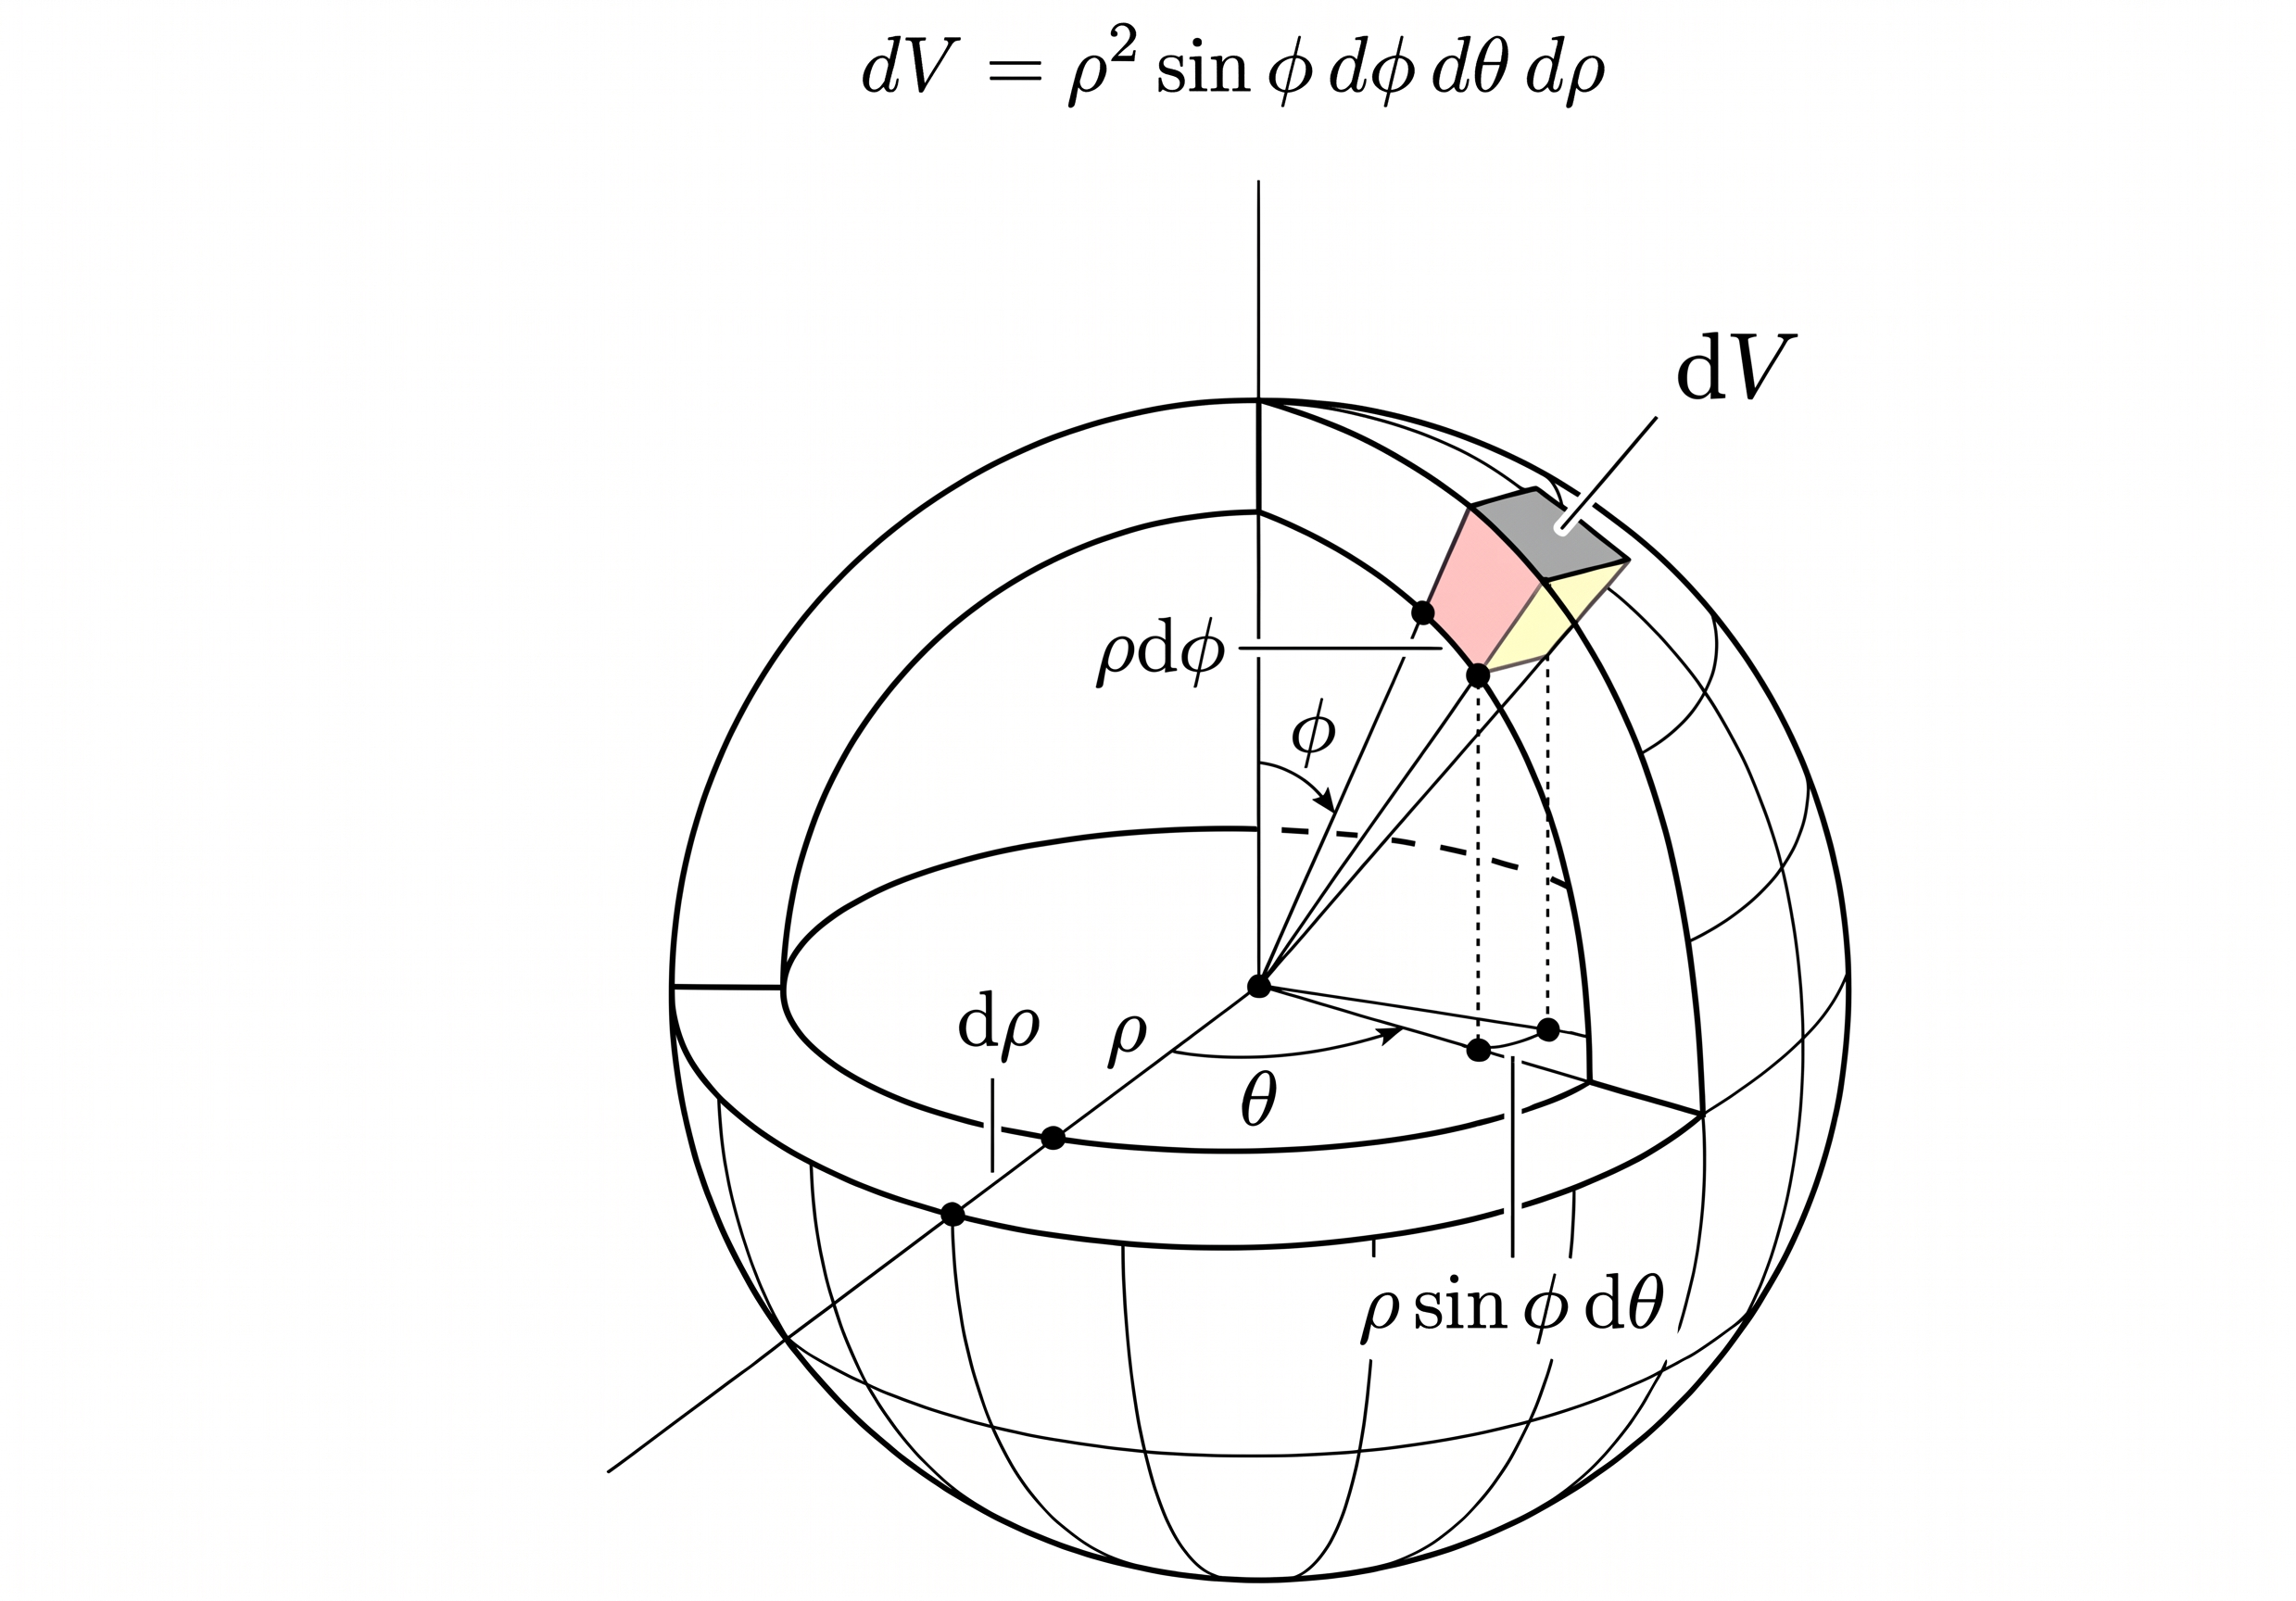
\includegraphics[width=0.8\textwidth]{figures/Spherical_Volume.png}
\caption{The spherical volume element is bounded by small changes in \(\rho\), \(\theta\), and \(\phi\).}
\label{fig:spherical_volume_element}
\end{figure}

Now find the small volume element.

A small spherical coordinate box has three side lengths, approximately:

\[
    d\rho
\]
in the radial direction,

\[
    \rho\,d\phi
\]
in the direction that changes \(\phi\), and

\[
    \rho\sin\phi\,d\theta
\]
in the direction that goes around the \(z\)-axis.



Multiplying these gives
\[
    dV
    =
    d\rho\cdot \rho\,d\phi\cdot \rho\sin\phi\,d\theta.
\]
So
\[
\boxed{
    dV=\rho^2\sin\phi\,d\rho\,d\phi\,d\theta.
}
\]


The factor \(\rho^2\) says that shells farther from the origin are larger.  The factor
\(\sin\phi\) says that angular pieces shrink near the poles.  Near \(\phi=0\), all values
of \(\theta\) crowd around the positive \(z\)-axis.

In form language, the same scale factor is
\[
\boxed{
    dx\wedge dy\wedge dz
    =
    \rho^2\sin\phi\,
    d\rho\wedge d\phi\wedge d\theta.
}
\]
For positive volume, we write
\[
    dV=\rho^2\sin\phi\,d\rho\,d\phi\,d\theta.
\]

\begin{example}[Volume of a ball]
Let \(B\) be the ball of radius \(4\) centered at the origin:
\[
    x^2+y^2+z^2\le16.
\]
In spherical coordinates, this is simply
\[
    0\le\rho\le4,\qquad
    0\le\phi\le\pi,\qquad
    0\le\theta\le2\pi.
\]
Therefore
\[
\begin{aligned}
\operatorname{Volume}(B)
&=
\int_0^{2\pi}\int_0^\pi\int_0^4
\rho^2\sin\phi\,d\rho\,d\phi\,d\theta\\
&=
\left(\int_0^{2\pi}d\theta\right)
\left(\int_0^\pi\sin\phi\,d\phi\right)
\left(\int_0^4\rho^2\,d\rho\right)\\
&=
(2\pi)(2)\left(\frac{64}{3}\right)\\
&=
\frac{256\pi}{3}.
\end{aligned}
\]
This matches
\[
    \frac43\pi(4)^3=\frac{256\pi}{3}.
\]
\end{example}

Again, the scale factor is not optional.  If we computed the unit ball without
\(\sin\phi\), we would get
\[
    \int_0^{2\pi}\int_0^\pi\int_0^1 \rho^2\,d\rho\,d\phi\,d\theta
    =
    \frac{2\pi^2}{3},
\]
not
\[
    \frac{4\pi}{3}.
\]
The missing \(\sin\phi\) would give too much weight to tiny angular pieces near the
poles.

\subsection{Balls, shells, and cones}

Spherical coordinates turn spheres into constant-\(\rho\) surfaces:
\[
    x^2+y^2+z^2=a^2
    \qquad\Longleftrightarrow\qquad
    \rho=a.
\]
So balls and shells become very simple.

\begin{example}[A spherical shell]
The shell between radius \(2\) and radius \(5\) is
\[
    2\le\rho\le5.
\]
With full angular range,
\[
    0\le\phi\le\pi,\qquad 0\le\theta\le2\pi.
\]
Its volume is
\[
\begin{aligned}
V
&=
\int_0^{2\pi}\int_0^\pi\int_2^5
\rho^2\sin\phi\,d\rho\,d\phi\,d\theta\\
&=
(2\pi)(2)\left[\frac{\rho^3}{3}\right]_2^5\\
&=
4\pi\cdot\frac{125-8}{3}\\
&=
156\pi.
\end{aligned}
\]
\end{example}

Cones also become simple, because a cone with vertex at the origin is a constant-angle
surface.  For example,
\[
    z=\sqrt{x^2+y^2}
\]
becomes
\[
    \rho\cos\phi=\rho\sin\phi.
\]
Away from the origin, this gives
\[
    \cos\phi=\sin\phi,
\]
so
\[
    \phi=\frac{\pi}{4}.
\]
The inside of the upper cone is
\[
    0\le\phi\le\frac{\pi}{4}.
\]

\begin{example}[A ball cut by a cone]
Find the volume inside the sphere
\[
    \rho\le3
\]
and inside the upper cone
\[
    z\ge \sqrt{x^2+y^2}.
\]
The cone is
\[
    0\le\phi\le\frac{\pi}{4}.
\]
The full rotation around the \(z\)-axis gives
\[
    0\le\theta\le2\pi.
\]
So
\[
\begin{aligned}
V
&=
\int_0^{2\pi}\int_0^{\pi/4}\int_0^3
\rho^2\sin\phi\,d\rho\,d\phi\,d\theta\\
&=
(2\pi)
\left(1-\cos\frac{\pi}{4}\right)
\left(9\right)\\
&=
18\pi\left(1-\frac{\sqrt2}{2}\right).
\end{aligned}
\]
Thus
\[
\boxed{
    V=18\pi\left(1-\frac{\sqrt2}{2}\right).
}
\]
\end{example}

A sphere fixes \(\rho\).  A cone fixes \(\phi\).  A vertical half-plane fixes \(\theta\).
That is the basic geometry of spherical bounds.

\subsection{Choosing the angular bounds}

The angle \(\theta\) is the same azimuth angle used in cylindrical coordinates.  It
describes the shadow in the \(xy\)-plane.

The angle \(\phi\) describes how far down from the positive \(z\)-axis the point lies.
It controls vertical opening.

\[
\begin{array}{c|c}
\text{condition} & \text{spherical meaning} \\ \hline
z\ge0 & 0\le\phi\le\pi/2\\[1mm]
z\le0 & \pi/2\le\phi\le\pi\\[1mm]
x\ge0,\ y\ge0 & 0\le\theta\le\pi/2\\[1mm]
\rho\le a & \text{inside sphere of radius }a\\[1mm]
z=\sqrt{x^2+y^2} & \phi=\pi/4
\end{array}
\]

\begin{example}[The first octant of a ball]
The first octant means
\[
    x\ge0,\qquad y\ge0,\qquad z\ge0.
\]
For the ball
\[
    \rho\le4,
\]
the bounds are
\[
    0\le\rho\le4,
    \qquad
    0\le\phi\le\frac{\pi}{2},
    \qquad
    0\le\theta\le\frac{\pi}{2}.
\]
The volume is
\[
\begin{aligned}
V
&=
\int_0^{\pi/2}\int_0^{\pi/2}\int_0^4
\rho^2\sin\phi\,d\rho\,d\phi\,d\theta\\
&=
\left(\frac{\pi}{2}\right)(1)\left(\frac{64}{3}\right)\\
&=
\frac{32\pi}{3}.
\end{aligned}
\]
This is one eighth of the full ball volume
\[
    \frac{256\pi}{3}.
\]
\end{example}

Spherical coordinates can also describe caps, where the radial lower bound is not zero.

\begin{example}[A spherical cap]
Find the volume inside the sphere
\[
    \rho\le3
\]
and above the plane
\[
    z=1.
\]
The plane becomes
\[
    \rho\cos\phi=1.
\]
Along a ray with angle \(\phi\), the plane is reached at
\[
    \rho=\sec\phi.
\]
For the ray to reach the sphere after crossing the plane, we need
\[
    \sec\phi\le3,
\]
or
\[
    \cos\phi\ge\frac13.
\]
Thus
\[
    0\le\phi\le\arccos\frac13.
\]
The bounds are
\[
    0\le\theta\le2\pi,
    \qquad
    0\le\phi\le\arccos\frac13,
    \qquad
    \sec\phi\le\rho\le3.
\]
So
\[
\boxed{
V=
\int_0^{2\pi}
\int_0^{\arccos(1/3)}
\int_{\sec\phi}^{3}
\rho^2\sin\phi\,d\rho\,d\phi\,d\theta.
}
\]
Compute:
\[
\begin{aligned}
V
&=
2\pi\int_0^{\arccos(1/3)}
\left[\frac{\rho^3}{3}\right]_{\sec\phi}^3
\sin\phi\,d\phi\\
&=
2\pi\int_0^{\arccos(1/3)}
\left(9-\frac13\sec^3\phi\right)\sin\phi\,d\phi.
\end{aligned}
\]
Let
\[
    \alpha=\arccos\frac13.
\]
Then
\[
    \cos\alpha=\frac13,
    \qquad
    \tan^2\alpha=8.
\]
Also,
\[
    \int_0^\alpha 9\sin\phi\,d\phi
    =
    9(1-\cos\alpha)=6,
\]
and
\[
    \frac13\int_0^\alpha \sec^3\phi\sin\phi\,d\phi
    =
    \frac13\int_0^\alpha \tan\phi\,\sec^2\phi\,d\phi
    =
    \frac16\tan^2\alpha
    =
    \frac43.
\]
Therefore
\[
    V=2\pi\left(6-\frac43\right)=\frac{28\pi}{3}.
\]
\end{example}

The angular bounds come from looking along rays from the origin.  A ray either enters
the solid immediately, enters after crossing a surface, or misses the solid.  Spherical
coordinates make us answer that ray question.

\subsection{Applications to gravitational and radial densities}

Many three-dimensional densities depend only on distance from a central point.  A
planet model, a gas cloud, and a radially symmetric charge distribution all have this
shape:
\[
    \delta=\delta(\rho).
\]
For a ball of radius \(a\), the total mass is
\[
\begin{aligned}
M
&=
\int_0^{2\pi}\int_0^\pi\int_0^a
\delta(\rho)\rho^2\sin\phi\,d\rho\,d\phi\,d\theta\\
&=
4\pi\int_0^a \delta(\rho)\rho^2\,d\rho.
\end{aligned}
\]
So
\[
\boxed{
    M=4\pi\int_0^a \delta(\rho)\rho^2\,d\rho.
}
\]
The angular part contributes \(4\pi\), and the radial part carries the real information.

\begin{example}[A simple model planet]
Suppose a planet has radius \(3\), and its density decreases linearly with distance from
the center:
\[
    \delta(\rho)=6-\rho,
    \qquad 0\le\rho\le3.
\]
Then
\[
\begin{aligned}
M
&=
4\pi\int_0^3(6-\rho)\rho^2\,d\rho\\
&=
4\pi\int_0^3(6\rho^2-\rho^3)\,d\rho\\
&=
4\pi\left[2\rho^3-\frac{\rho^4}{4}\right]_0^3\\
&=
4\pi\left(54-\frac{81}{4}\right)\\
&=
135\pi.
\end{aligned}
\]
Thus
\[
\boxed{
    M=135\pi.
}
\]
\end{example}

The same scale factor explains a familiar feature of inverse-square laws.  Suppose an
energy density in a spherical shell is
\[
    u(\rho)=\frac{10}{\rho^2},
    \qquad 1\le\rho\le4.
\]
The total energy in the shell is
\[
\begin{aligned}
E
&=
\int_0^{2\pi}\int_0^\pi\int_1^4
\frac{10}{\rho^2}\rho^2\sin\phi\,d\rho\,d\phi\,d\theta\\
&=
10(2\pi)(2)\int_1^4 d\rho\\
&=
120\pi.
\end{aligned}
\]
The \(\rho^2\) in the volume element cancels the \(1/\rho^2\) in the density.  Each
unit of radial thickness contributes the same amount.  Later, when we study flux, the
same geometric growth of spherical area will help explain why gravitational and electric
fields often have inverse-square form.

Cylindrical and spherical coordinates changed the shape of \(dV\), but not the meaning
of the integral.  A triple integral still adds tiny contributions through a solid.  Once we
can add density, the next questions are natural: Where is the mass balanced?  How far
is it spread from an axis?  How much charge or energy does the solid contain?  Those
are the applications that turn triple integrals from volume machines into physical
measuring tools.
\section{Applications of triple integrals}
\label{sec:11.5}

Sections \ref{sec:11.1}--\ref{sec:11.4} taught us how to add over a solid.  The
geometry changed from boxes to wedges, cylinders, cones, balls, and shells, but the
basic contribution always had the same shape:
\[
    \text{value near a point}\times \text{tiny volume}.
\]
Now the value near the point becomes physical.  It may be mass density, charge
density, energy density, or probability density.

Because spherical coordinates already use the letter \(\rho\), this section writes mass
density as
\[
    \delta(x,y,z).
\]

\subsection{Mass and density in space}

Imagine a clear gel block in a laboratory.  A chemical additive has settled unevenly, so
the density is larger near the top.  The block occupies
\[
    E=[0,4]\times[0,3]\times[0,2],
\]
and its density is
\[
    \delta(x,y,z)=2+z
\]
grams per cubic centimeter.

A small box near \((x,y,z)\) has mass approximately
\[
    \delta(x,y,z)\,\Delta V.
\]
Adding all those small masses gives
\[
    M=\iiint_E \delta(x,y,z)\,dV.
\]
For this block,
\[
\begin{aligned}
M
&=
\int_0^4\int_0^3\int_0^2 (2+z)\,dz\,dy\,dx\\
&=
\int_0^4\int_0^3
\left[2z+\frac{z^2}{2}\right]_0^2
\,dy\,dx\\
&=
\int_0^4\int_0^3 6\,dy\,dx\\
&=
72.
\end{aligned}
\]
So the total mass is
\[
\boxed{
    M=72.
}
\]

\begin{definition}[Mass from a density]
If a solid \(E\) has mass density
\[
    \delta(x,y,z),
\]
then its mass is
\[
\boxed{
    M=\iiint_E \delta(x,y,z)\,dV.
}
\]
\end{definition}

In oriented form notation, the same integral can be written
\[
    \iiint_E \delta(x,y,z)\,dx\wedge dy\wedge dz,
\]
when the solid is given the standard orientation.  For mass, however, we usually write
\(dV\), because mass uses positive volume.

\begin{example}[Mass of a cone with density depending on height]
A solid cone has height \(4\), radius \(4\), and density
\[
    \delta(x,y,z)=1+z.
\]
The cone has equation
\[
    0\le z\le 4-r
\]
in cylindrical coordinates.  Thus
\[
    0\le \theta\le 2\pi,
    \qquad
    0\le r\le4,
    \qquad
    0\le z\le4-r.
\]
The mass is
\[
\begin{aligned}
M
&=
\int_0^{2\pi}\int_0^4\int_0^{4-r}
(1+z)r\,dz\,dr\,d\theta\\
&=
2\pi\int_0^4
\left[z+\frac{z^2}{2}\right]_0^{4-r}
r\,dr\\
&=
2\pi\int_0^4
\left((4-r)+\frac12(4-r)^2\right)r\,dr.
\end{aligned}
\]
Expand:
\[
    (4-r)+\frac12(4-r)^2
    =
    4-r+8-4r+\frac12r^2
    =
    12-5r+\frac12r^2.
\]
So
\[
\begin{aligned}
M
&=
2\pi\int_0^4
\left(12r-5r^2+\frac12r^3\right)\,dr\\
&=
2\pi
\left[
6r^2-\frac53r^3+\frac18r^4
\right]_0^4\\
&=
2\pi
\left(
96-\frac{320}{3}+32
\right)\\
&=
2\pi\cdot\frac{64}{3}\\
&=
\frac{128\pi}{3}.
\end{aligned}
\]
Thus
\[
\boxed{
    M=\frac{128\pi}{3}.
}
\]
\end{example}

The density decides how much each small volume piece counts.  The geometry decides
where the pieces are.

\subsection{Center of mass}

Mass tells us how much matter there is.  The center of mass tells us where that matter
balances.

Return to the gel block
\[
    E=[0,4]\times[0,3]\times[0,2],
\]
with density
\[
    \delta(x,y,z)=2+z.
\]
The density depends only on height.  So symmetry already tells us
\[
    \bar x=2,
    \qquad
    \bar y=\frac32.
\]
But the \(z\)-coordinate of the center should be above the geometric middle \(z=1\),
because the block is denser near the top.

To find it, we compute the first moments:
\[
    N_x=\iiint_E x\delta\,dV,
    \qquad
    N_y=\iiint_E y\delta\,dV,
    \qquad
    N_z=\iiint_E z\delta\,dV.
\]
For this block,
\[
\begin{aligned}
N_x
&=
\int_0^4\int_0^3\int_0^2 x(2+z)\,dz\,dy\,dx\\
&=
\left(\int_0^4 x\,dx\right)
\left(\int_0^3 dy\right)
\left(\int_0^2(2+z)\,dz\right)\\
&=
8\cdot3\cdot6\\
&=
144.
\end{aligned}
\]
Similarly,
\[
\begin{aligned}
N_y
&=
\left(\int_0^4 dx\right)
\left(\int_0^3 y\,dy\right)
\left(\int_0^2(2+z)\,dz\right)\\
&=
4\cdot\frac92\cdot6\\
&=
108.
\end{aligned}
\]
For the height moment,
\[
\begin{aligned}
N_z
&=
\int_0^4\int_0^3\int_0^2 z(2+z)\,dz\,dy\,dx\\
&=
12\int_0^2(2z+z^2)\,dz\\
&=
12\left[z^2+\frac{z^3}{3}\right]_0^2\\
&=
12\left(4+\frac83\right)\\
&=
80.
\end{aligned}
\]
Since \(M=72\), the center of mass is
\[
\boxed{
    (\bar x,\bar y,\bar z)
    =
    \left(
    \frac{N_x}{M},\frac{N_y}{M},\frac{N_z}{M}
    \right)
    =
    \left(2,\frac32,\frac{10}{9}\right).
}
\]
As expected,
\[
    \bar z=\frac{10}{9}>1.
\]

\begin{figure}[h]
\centering
\begin{tikzpicture}[scale=0.8, >=stealth]
    \coordinate (O) at (0,0);
    \coordinate (A) at (4,0);
    \coordinate (B) at (5.2,1.1);
    \coordinate (C) at (1.2,1.1);
    \coordinate (D) at (0,2.6);
    \coordinate (E) at (4,2.6);
    \coordinate (F) at (5.2,3.7);
    \coordinate (G) at (1.2,3.7);

    \draw[fill=gray!8, thick] (O)--(A)--(B)--(C)--cycle;
    \draw[fill=gray!15, thick] (D)--(E)--(F)--(G)--cycle;
    \draw[thick] (O)--(D);
    \draw[thick] (A)--(E);
    \draw[thick] (B)--(F);
    \draw[thick] (C)--(G);

    \foreach \z/\shade in {0.45/10,0.9/16,1.35/23,1.8/30,2.25/38} {
        \draw[fill=blue!\shade, draw=none, opacity=0.45]
            (0,\z) -- (4,\z) -- (5.2,{1.1+\z}) -- (1.2,{1.1+\z}) -- cycle;
    }

    \fill[red!70!black] (2.67,1.92) circle (3pt);
    \node[right] at (2.75,1.92) {center of mass};

    \node at (2,-0.55) {\(x\)-direction};
    \node[left] at (0,1.3) {\(z\)};
    \node at (2.6,-1.05) {denser layers near the top raise \(\bar z\)};
\end{tikzpicture}
\caption{When density increases with height, the center of mass moves upward.}
\end{figure}

\begin{definition}[Center of mass in space]
Let \(E\) be a solid with density \(\delta(x,y,z)\), and suppose
\[
    M=\iiint_E \delta\,dV>0.
\]
Define the first moments
\[
    N_x=\iiint_E x\delta\,dV,
    \qquad
    N_y=\iiint_E y\delta\,dV,
    \qquad
    N_z=\iiint_E z\delta\,dV.
\]
Then the center of mass is
\[
\boxed{
    (\bar x,\bar y,\bar z)
    =
    \left(
        \frac{N_x}{M},
        \frac{N_y}{M},
        \frac{N_z}{M}
    \right).
}
\]
\end{definition}

The condition \(M>0\) matters.  A real mass density is nonnegative, and if there is any
material at all, then \(M>0\).  But for signed quantities, such as electric charge, the
same formula can break.

\begin{example}[Why positive total mass is needed]
Suppose a cube contains equal amounts of positive and negative charge.  A signed
charge density \(q\) might satisfy
\[
    \iiint_E q\,dV=0.
\]
The expression
\[
    \frac{\iiint_E xq\,dV}{\iiint_E q\,dV}
\]
then tries to divide by zero.  There may be a meaningful center of positive charge and a
meaningful center of negative charge, but there is no center of ``total signed charge''
given by this quotient.

So the center of mass formula belongs to a positive finite mass distribution.
\end{example}

\subsection{Moment of inertia}

Center of mass measures balance.  Moment of inertia measures resistance to rotation.

A point mass far from an axis is harder to spin than the same point mass near the axis.
The distance is squared, so far-away material counts strongly.

If a small volume piece has mass
\[
    \delta\,dV
\]
and its distance from the axis is \(s\), then its small contribution to moment of inertia
is
\[
    s^2\delta\,dV.
\]

\begin{definition}[Moment of inertia about an axis]
For a solid \(E\) with density \(\delta(x,y,z)\), the moment of inertia about an axis
is
\[
\boxed{
    I=\iiint_E s^2\delta(x,y,z)\,dV,
}
\]
where \(s\) is the distance from \((x,y,z)\) to the axis.
\end{definition}

For the coordinate axes,
\[
\boxed{
    I_x=\iiint_E (y^2+z^2)\delta\,dV,
}
\]
\[
\boxed{
    I_y=\iiint_E (x^2+z^2)\delta\,dV,
}
\]
and
\[
\boxed{
    I_z=\iiint_E (x^2+y^2)\delta\,dV.
}
\]

\begin{example}[A solid cylinder spinning around its axis]
A solid cylinder has radius \(2\), height \(3\), and constant density \(5\).  It spins
around its central \(z\)-axis.

In cylindrical coordinates,
\[
    0\le r\le2,
    \qquad
    0\le\theta\le2\pi,
    \qquad
    0\le z\le3.
\]
The distance to the \(z\)-axis is
\[
    s=r.
\]
So
\[
\begin{aligned}
I_z
&=
\int_0^{2\pi}\int_0^2\int_0^3
r^2\cdot 5\cdot r\,dz\,dr\,d\theta\\
&=
5\int_0^{2\pi}\int_0^2\int_0^3
r^3\,dz\,dr\,d\theta\\
&=
5(2\pi)(3)\int_0^2 r^3\,dr\\
&=
30\pi\left[\frac{r^4}{4}\right]_0^2\\
&=
30\pi\cdot4\\
&=
120\pi.
\end{aligned}
\]
Thus
\[
\boxed{
    I_z=120\pi.
}
\]

The mass of the cylinder is
\[
    M=5\pi(2)^2(3)=60\pi.
\]
So
\[
    I_z=\frac12M(2)^2,
\]
which matches the familiar physics formula for a solid cylinder.
\end{example}

\begin{figure}[h]
\centering
\begin{tikzpicture}[scale=0.9, >=stealth]
    % Define the symmetric horizontal shading (distance from vertical axis is |x|)
    \pgfdeclarehorizontalshading{densityshading}{100bp}{
        color(0bp)=(red!80!black);     % At x = -R, color corresponds to (-R)^2
        color(25bp)=(red!40!white);    % Intermediate point for non-linear transition
        color(50bp)=(white);          % At x = 0 (axis), color is minimal
        color(75bp)=(red!40!white);    % Non-linear intermediate
        color(100bp)=(red!80!black)    % At x = +R, color is max
    }

    % Fill the circle with the custom shading
    \begin{scope}
        \clip (0,0) circle (2.5);
        \shade[shading=densityshading, shading angle=0] (-2.5,-2.5) rectangle (2.5,2.5);
    \end{scope}

    % Boundary circle and guidelinles
    \draw[thick] (0,0) circle (2.5);
    \draw[gray!40, thin] (0,0) circle (0.8); % Gray slightly darkened for contrast
    \draw[gray!40, thin] (0,0) circle (1.6);

    % Axes and point with vector
    \draw[->] (-3.2,0) -- (3.4,0) node[right] {\(x\)};
    \draw[->] (0,-3.2) -- (0,3.4) node[above] {\(y\)};
    
    \draw[->, thick] (0,0) -- (35:1.7) node[midway, above] {\(r\)};
    \fill (35:1.7) circle (2pt);

    % Main axis line
    \draw[very thick, blue!60!black] (0,-3) -- (0,3);
    \node[blue!60!black, left] at (0,2.9) {axis};

    % Descriptive label
    \node at (0,-3.8) {material farther from the axis contributes \(r^2\) times as much};
\end{tikzpicture}
\caption{For rotation about the \(z\)-axis, the distance factor is \(r^2=x^2+y^2\).}
\end{figure}

Moment of inertia is an integral because a solid is made of many tiny masses, each at
its own distance from the axis.

\subsection{Total charge and total energy}

Mass density is nonnegative.  Charge density can be positive or negative.  Energy
density is usually nonnegative.

If \(q(x,y,z)\) is charge density, then total charge is
\[
\boxed{
    Q=\iiint_E q(x,y,z)\,dV.
}
\]
If \(u(x,y,z)\) is energy density, then total energy is
\[
\boxed{
    \mathcal E=\iiint_E u(x,y,z)\,dV.
}
\]

\begin{example}[Positive and negative charge can cancel]
A charged cylinder has radius \(1\), height \(2\), and charge density
\[
    q(x,y,z)=z-1.
\]
The lower half has negative charge, and the upper half has positive charge.

In cylindrical coordinates,
\[
    0\le r\le1,
    \qquad
    0\le\theta\le2\pi,
    \qquad
    0\le z\le2.
\]
The total charge is
\[
\begin{aligned}
Q
&=
\int_0^{2\pi}\int_0^1\int_0^2
(z-1)r\,dz\,dr\,d\theta\\
&=
\left(\int_0^{2\pi}d\theta\right)
\left(\int_0^1 r\,dr\right)
\left(\int_0^2(z-1)\,dz\right).
\end{aligned}
\]
But
\[
    \int_0^2(z-1)\,dz
    =
    \left[\frac{z^2}{2}-z\right]_0^2
    =
    2-2
    =
    0.
\]
Therefore
\[
\boxed{
    Q=0.
}
\]
The cylinder is not uncharged everywhere.  Its total signed charge is zero because the
positive and negative parts cancel.
\end{example}

\begin{example}[Energy stored in a spherical battery material]
A ball of radius \(2\) has energy density depending only on distance from the center:
\[
    u(\rho)=10\left(1-\frac{\rho}{2}\right),
    \qquad
    0\le \rho\le2.
\]
The density is largest at the center and drops to \(0\) at the surface.

Using spherical coordinates,
\[
\begin{aligned}
\mathcal E
&=
\int_0^{2\pi}\int_0^\pi\int_0^2
10\left(1-\frac{\rho}{2}\right)\rho^2\sin\phi
\,d\rho\,d\phi\,d\theta\\
&=
4\pi\cdot10\int_0^2
\left(\rho^2-\frac12\rho^3\right)\,d\rho\\
&=
40\pi
\left[
\frac{\rho^3}{3}-\frac{\rho^4}{8}
\right]_0^2\\
&=
40\pi\left(\frac83-2\right)\\
&=
\frac{80\pi}{3}.
\end{aligned}
\]
So
\[
\boxed{
    \mathcal E=\frac{80\pi}{3}.
}
\]
\end{example}

The same triple integral notation covers mass, charge, and energy.  The units of the
integrand tell us what is being added.

\[
\begin{array}{c|c|c}
\text{Density} & \text{Units} & \text{Integral} \\ \hline
\delta(x,y,z) & \text{mass}/\text{volume} &
\displaystyle M=\iiint_E \delta\,dV \\[3mm]
q(x,y,z) & \text{charge}/\text{volume} &
\displaystyle Q=\iiint_E q\,dV \\[3mm]
u(x,y,z) & \text{energy}/\text{volume} &
\displaystyle \mathcal E=\iiint_E u\,dV
\end{array}
\]

\subsection{Probability in three dimensions}

A probability density is another kind of density.  Instead of mass per volume or charge
per volume, it gives probability per volume.

If a random point is chosen in a solid region \(E\), a probability density \(p(x,y,z)\)
must satisfy two conditions:
\[
    p(x,y,z)\ge0
\]
and
\[
    \iiint_E p(x,y,z)\,dV=1.
\]
Then the probability that the point lies in a smaller region \(A\subseteq E\) is
\[
\boxed{
    \operatorname{Prob}(A)=\iiint_A p(x,y,z)\,dV.
}
\]

\begin{example}[A random point more likely near the top of a box]
A random point is chosen in the unit cube
\[
    0\le x\le1,
    \qquad
    0\le y\le1,
    \qquad
    0\le z\le1.
\]
Suppose the density has the form
\[
    p(x,y,z)=C(1+z).
\]
First find \(C\).  We need
\[
    \iiint_E C(1+z)\,dV=1.
\]
Thus
\[
\begin{aligned}
1
&=
C\int_0^1\int_0^1\int_0^1(1+z)\,dz\,dy\,dx\\
&=
C\left[z+\frac{z^2}{2}\right]_0^1\\
&=
C\cdot\frac32.
\end{aligned}
\]
So
\[
\boxed{
    C=\frac23.
}
\]

Now find the probability that
\[
    z\le\frac12.
\]
This is
\[
\begin{aligned}
\operatorname{Prob}\left(z\le\frac12\right)
&=
\int_0^1\int_0^1\int_0^{1/2}
\frac23(1+z)\,dz\,dy\,dx\\
&=
\frac23
\left[z+\frac{z^2}{2}\right]_0^{1/2}\\
&=
\frac23\left(\frac12+\frac18\right)\\
&=
\frac{5}{12}.
\end{aligned}
\]
So
\[
\boxed{
    \operatorname{Prob}\left(z\le\frac12\right)=\frac{5}{12}.
}
\]
Even though the lower half of the cube has half the volume, it has less than half the
probability, because the density increases with \(z\).
\end{example}

The conditions
\[
    p\ge0,
    \qquad
    \iiint_E p\,dV=1
\]
are not cosmetic.  Without them, the word probability loses its meaning.

\begin{example}[Why probability densities must be nonnegative and normalized]
On the unit cube, the function
\[
    p(x,y,z)=2
\]
is nonnegative, but
\[
    \iiint_E 2\,dV=2.
\]
It assigns total probability \(2\), not \(1\), so it is not a probability density.

The function
\[
    q(x,y,z)=2z-1
\]
has total integral \(0\), and it is negative when \(z<1/2\).  It cannot describe
probability, because some regions would receive negative probability.

A probability density is an ordinary density with two extra promises: no negative
amounts, and total amount exactly \(1\).
\end{example}

This last example points beyond three dimensions.  A random point might have four
coordinates, or ten, or a hundred.  A gas molecule has position and velocity.  A data
point may have many measured features.  The adding idea does not stop at three
coordinates.  What changes is harder to draw: a tiny piece is no longer a rectangle or a
box we can picture.  It is still a product of tiny coordinate lengths.

\section{Higher-dimensional integrals}
\label{sec:11.6}

The probability example at the end of Section \ref{sec:11.5} did not really care that the
random point had three coordinates.  A system may have many coordinates:
\[
    x_1,x_2,\ldots,x_n.
\]
A triple integral is the case \(n=3\).  Higher-dimensional integrals follow the same
adding rule, but the pictures become less trustworthy.

The wedge notation in this book will stay in dimensions \(1\), \(2\), and \(3\).  In this
optional section, we write
\[
    dV_n
\]
for positive \(n\)-dimensional volume.

\subsection{What changes in \texorpdfstring{\(\mathbb R^n\)}{Rn}}

A point in \(\mathbb R^n\) is written
\[
    \mathbf x=(x_1,x_2,\ldots,x_n).
\]
A rectangular box in \(\mathbb R^n\) has the form
\[
    B=[a_1,b_1]\times[a_2,b_2]\times\cdots\times[a_n,b_n].
\]
Its side lengths are
\[
    b_1-a_1,\quad b_2-a_2,\quad \ldots,\quad b_n-a_n.
\]
Its \(n\)-dimensional volume is
\[
\boxed{
    \operatorname{Vol}_n(B)
    =
    (b_1-a_1)(b_2-a_2)\cdots(b_n-a_n).
}
\]

A small coordinate box has side lengths
\[
    \Delta x_1,\Delta x_2,\ldots,\Delta x_n.
\]
Its small volume is
\[
    \Delta V_n
    =
    \Delta x_1\Delta x_2\cdots\Delta x_n.
\]
So the Riemann sum for a function
\[
    f(x_1,\ldots,x_n)
\]
has the form
\[
    \sum f(\mathbf x_i^*)\,\Delta V_{n,i}.
\]
If these sums settle to a single value, we write
\[
\boxed{
    \int_E f(\mathbf x)\,dV_n.
}
\]

\begin{example}[A four-dimensional quality-control box]
A machine produces parts with four measured deviations:
\[
    x_1,\quad x_2,\quad x_3,\quad x_4.
\]
Suppose each deviation is allowed to lie between \(-1\) and \(1\).  The acceptable
region is the four-dimensional box
\[
    B=[-1,1]^4.
\]
Its volume is
\[
    \operatorname{Vol}_4(B)=2\cdot2\cdot2\cdot2=16.
\]

If all points in \(B\) are equally likely, the probability density is constant:
\[
    p=\frac1{16}.
\]
The probability that every deviation lies between \(-1/2\) and \(1/2\) is
\[
\begin{aligned}
\operatorname{Prob}\left([-1/2,1/2]^4\right)
&=
\int_{[-1/2,1/2]^4}\frac1{16}\,dV_4\\
&=
\frac1{16}\cdot
(1\cdot1\cdot1\cdot1)\\
&=
\frac1{16}.
\end{aligned}
\]
Each coordinate range was cut in half, but the four-dimensional volume was cut by
\[
    \left(\frac12\right)^4.
\]
This is the first hint that high-dimensional size shrinks faster than our eyes expect.
\end{example}

\begin{definition}[Higher-dimensional integral]
Let \(E\subseteq\mathbb R^n\).  If Riemann sums
\[
    \sum f(\mathbf x_i^*)\,\Delta V_{n,i}
\]
approach one number as the small \(n\)-dimensional boxes shrink, independent of the
sample points, then that number is the integral of \(f\) over \(E\):
\[
\boxed{
    \int_E f(\mathbf x)\,dV_n.
}
\]
\end{definition}

For \(n=1\), this is an ordinary single-variable integral.  For \(n=2\), it is a double
integral.  For \(n=3\), it is a triple integral.

\subsection{Product regions and Fubini's theorem}

The easiest higher-dimensional regions are boxes and product regions, because each
coordinate has its own interval.

For example, let
\[
    B=[0,2]\times[0,3]\times[0,1]\times[0,4].
\]
Then
\[
    \operatorname{Vol}_4(B)=2\cdot3\cdot1\cdot4=24.
\]

Now compute
\[
    I=\int_B (x_1+x_4)\,dV_4.
\]
Using iterated integrals,
\[
\begin{aligned}
I
&=
\int_0^2\int_0^3\int_0^1\int_0^4
(x_1+x_4)\,dx_4\,dx_3\,dx_2\,dx_1.
\end{aligned}
\]
Split the integral into two pieces:
\[
    I
    =
    \int_B x_1\,dV_4+\int_B x_4\,dV_4.
\]
For the \(x_1\)-piece,
\[
\begin{aligned}
\int_B x_1\,dV_4
&=
\left(\int_0^2 x_1\,dx_1\right)
\left(\int_0^3 dx_2\right)
\left(\int_0^1 dx_3\right)
\left(\int_0^4 dx_4\right)\\
&=
2\cdot3\cdot1\cdot4\\
&=
24.
\end{aligned}
\]
For the \(x_4\)-piece,
\[
\begin{aligned}
\int_B x_4\,dV_4
&=
\left(\int_0^2 dx_1\right)
\left(\int_0^3 dx_2\right)
\left(\int_0^1 dx_3\right)
\left(\int_0^4 x_4\,dx_4\right)\\
&=
2\cdot3\cdot1\cdot8\\
&=
48.
\end{aligned}
\]
Thus
\[
\boxed{
    I=72.
}
\]
The average value of \(x_1+x_4\) over the box is
\[
    \frac{72}{24}=3.
\]
That is the average of \(x_1\), which is \(1\), plus the average of \(x_4\), which is
\(2\).

\begin{theorem}[Fubini's theorem for boxes in \(\mathbb R^n\)]
Let
\[
    B=[a_1,b_1]\times\cdots\times[a_n,b_n],
\]
and suppose \(f\) is continuous on \(B\).  Then
\[
\boxed{
    \int_B f(\mathbf x)\,dV_n
}
\]
can be computed as an iterated integral in any order.

For example,
\[
\boxed{
\int_B f\,dV_n
=
\int_{a_1}^{b_1}\cdots\int_{a_n}^{b_n}
f(x_1,\ldots,x_n)\,dx_n\cdots dx_1.
}
\]
\end{theorem}

Continuity is a safe condition.  It is stronger than necessary, but it keeps the adding
process well-behaved.

\begin{example}[A nonintegrable function still breaks the story]
On the unit box
\[
    [0,1]^n,
\]
define
\[
    q(x_1,\ldots,x_n)
    =
    \begin{cases}
    1, & x_1\text{ is rational},\\
    0, & x_1\text{ is irrational}.
    \end{cases}
\]
Every small \(n\)-dimensional box contains points with rational \(x_1\) and points with
irrational \(x_1\).  The upper sums are always \(1\), and the lower sums are always
\(0\).

So the Riemann integral does not exist.  Fubini's theorem cannot rescue an integral
that was never there.
\end{example}

There is a useful special case when the function factors.  If
\[
    f(x_1,\ldots,x_n)=g_1(x_1)g_2(x_2)\cdots g_n(x_n),
\]
then on a box,
\[
\boxed{
    \int_B f\,dV_n
    =
    \left(\int_{a_1}^{b_1}g_1(x_1)\,dx_1\right)
    \cdots
    \left(\int_{a_n}^{b_n}g_n(x_n)\,dx_n\right).
}
\]
The integral separates because the variables separate.

\begin{example}[A separated density]
Let
\[
    f(x_1,x_2,x_3,x_4)=e^{-x_1}(1+x_2)x_3^2
\]
on
\[
    [0,1]\times[0,2]\times[0,3]\times[0,4].
\]
The function does not depend on \(x_4\), so the \(x_4\)-integral contributes a factor
of \(4\).  We get
\[
\begin{aligned}
\int f\,dV_4
&=
\left(\int_0^1e^{-x_1}\,dx_1\right)
\left(\int_0^2(1+x_2)\,dx_2\right)
\left(\int_0^3x_3^2\,dx_3\right)
\left(\int_0^4 dx_4\right)\\
&=
(1-e^{-1})(4)(9)(4)\\
&=
144(1-e^{-1}).
\end{aligned}
\]
\end{example}

The arithmetic looks familiar because Fubini turns one higher-dimensional adding
problem into several one-dimensional ones.

\subsection{Volumes of higher-dimensional balls and boxes}

Boxes are easy in every dimension:
\[
    \operatorname{Vol}_n([0,L]^n)=L^n.
\]
Balls are subtler.

The \(n\)-dimensional ball of radius \(R\) is
\[
    B_n(R)=
    \left\{
    (x_1,\ldots,x_n):
    x_1^2+\cdots+x_n^2\le R^2
    \right\}.
\]
For the first few dimensions:
\[
\begin{array}{c|c|c}
n & B_n(R) & \operatorname{Vol}_n(B_n(R)) \\ \hline
1 & \text{interval} & 2R\\[1mm]
2 & \text{disk} & \pi R^2\\[1mm]
3 & \text{solid ball} & \dfrac43\pi R^3
\end{array}
\]

The four-dimensional ball cannot be drawn, but it can be sliced.

Let
\[
    B_4(1)=
    \{(x,y,z,w):x^2+y^2+z^2+w^2\le1\}.
\]
Fix \(w\).  Then the remaining variables satisfy
\[
    x^2+y^2+z^2\le1-w^2.
\]
That is a three-dimensional ball of radius
\[
    \sqrt{1-w^2}.
\]
Its volume is
\[
    \frac43\pi(1-w^2)^{3/2}.
\]
So
\[
\begin{aligned}
\operatorname{Vol}_4(B_4(1))
&=
\int_{-1}^{1}
\frac43\pi(1-w^2)^{3/2}\,dw.
\end{aligned}
\]
Use
\[
    w=\sin u.
\]
Then
\[
    dw=\cos u\,du,
    \qquad
    (1-w^2)^{3/2}=\cos^3u,
\]
and \(u\) runs from \(-\pi/2\) to \(\pi/2\).  Therefore
\[
\begin{aligned}
\operatorname{Vol}_4(B_4(1))
&=
\frac43\pi
\int_{-\pi/2}^{\pi/2}\cos^4u\,du.
\end{aligned}
\]
Since
\[
    \cos^4u=\frac{3+4\cos(2u)+\cos(4u)}{8},
\]
we have
\[
    \int_{-\pi/2}^{\pi/2}\cos^4u\,du=\frac{3\pi}{8}.
\]
Thus
\[
\boxed{
    \operatorname{Vol}_4(B_4(1))
    =
    \frac43\pi\cdot\frac{3\pi}{8}
    =
    \frac{\pi^2}{2}.
}
\]

Scaling by \(R\) in all four coordinates multiplies four-dimensional volume by
\(R^4\).  So
\[
\boxed{
    \operatorname{Vol}_4(B_4(R))
    =
    \frac{\pi^2}{2}R^4.
}
\]

The pattern continues:
\[
\begin{array}{c|c}
n & \operatorname{Vol}_n(B_n(R)) \\ \hline
1 & 2R\\[1mm]
2 & \pi R^2\\[1mm]
3 & \dfrac43\pi R^3\\[2mm]
4 & \dfrac{\pi^2}{2}R^4\\[2mm]
5 & \dfrac{8\pi^2}{15}R^5
\end{array}
\]

The formula has a compact version involving the gamma function, but the main idea is
already visible: higher-dimensional balls can be studied by slicing them into
lower-dimensional balls.

\subsection{Why high-dimensional geometry feels surprising}

High-dimensional geometry often disagrees with three-dimensional intuition.  The
reason is not mysterious.  Powers grow and shrink quickly.

For an \(n\)-dimensional ball, scaling the radius by \(a\) scales volume by
\[
    a^n.
\]
So the ball of half the radius has volume fraction
\[
\boxed{
    \left(\frac12\right)^n.
}
\]
In three dimensions, that fraction is
\[
    \frac18.
\]
In ten dimensions, it is
\[
    \frac1{1024}.
\]
In one hundred dimensions, it is
\[
    2^{-100}.
\]
So in high dimensions, very little of a ball's volume lies near the center.  Most of it
sits close to the outer shell.

The cube gives another surprise.  The cube
\[
    [-1,1]^n
\]
has volume
\[
    2^n.
\]
Its corners have distance
\[
    \sqrt{1^2+1^2+\cdots+1^2}=\sqrt n
\]
from the origin.  As \(n\) grows, the corners move farther and farther away, even
though every coordinate still lies between \(-1\) and \(1\).

In four dimensions, the ball of radius \(1\) inside the cube \([-1,1]^4\) has volume
\[
    \frac{\pi^2}{2}.
\]
The cube has volume
\[
    16.
\]
So the fraction occupied by the ball is
\[
    \frac{\pi^2/2}{16}
    =
    \frac{\pi^2}{32}
    \approx 0.31.
\]
Already by dimension \(4\), much of the cube lies outside the inscribed ball, toward
the corners.

These facts matter in probability, statistics, data science, and physics.  A point with
many coordinates does not behave like a point in a drawing.  Volume migrates toward
boundaries, corners, and shells.

But the integral itself has not changed.  It still adds tiny contributions.  The hard
part is describing how a small coordinate box in one system becomes a small piece in
another system.  We have already met two answers:
\[
    dV=r\,dr\,d\theta\,dz
\]
and
\[
    dV=\rho^2\sin\phi\,d\rho\,d\phi\,d\theta.
\]
Those factors were not tricks for cylinders and spheres.  They are examples of a
single rule.  Chapter \ref{ch:12} finds that rule by looking at how a coordinate map
stretches tiny boxes, and the determinant returns as the scale factor.
\section{Chapter review and applications}
\label{sec:11.7}

Chapter \ref{ch:11} took the adding idea one dimension higher.  A double integral
adds over a region in the plane:
\[
    f(x,y)\,dA.
\]
A triple integral adds over a solid:
\[
    f(x,y,z)\,dV.
\]
The tiny pieces changed from rectangles to boxes.  The story did not change:
\[
    \text{value near a point}\times \text{tiny volume}.
\]

The hard part is rarely the antiderivative.  The hard part is describing the solid without
counting too much or too little.

\subsection{Skills: triple integrals in several coordinate systems}

A triple integral begins with one question:
\[
    \text{What solid am I adding over?}
\]
After that, the coordinate system should serve the geometry.

\begin{figure}[h]
\centering
\begin{tikzpicture}[scale=0.88, >=stealth]
    \node[draw, rounded corners, align=center, minimum width=4.4cm, minimum height=0.9cm]
        (start) at (0,0) {Triple integral\\ \(\displaystyle \iiint_E f\,dV\)};

    % Widened from -5.2 to -5.9
    \node[draw, rounded corners, align=center, minimum width=4.4cm, minimum height=0.9cm]
        (rect) at (-5.9,-2) {Boxes, wedges, slabs\\ rectangular coordinates};

    \node[draw, rounded corners, align=center, minimum width=4.4cm, minimum height=0.9cm]
        (cyl) at (0,-2) {Cylinders, cones, tubes\\ cylindrical coordinates};

    % Widened from 5.2 to 5.9
    \node[draw, rounded corners, align=center, minimum width=4.4cm, minimum height=0.9cm]
        (sph) at (5.9,-2) {Balls, shells, central symmetry\\ spherical coordinates};

    \node[draw, rounded corners, align=center, minimum width=4.4cm, minimum height=0.9cm]
        (app) at (-2.8,-4.5) {Mass, charge, energy,\\ probability};

    \node[draw, rounded corners, align=center, minimum width=4.4cm, minimum height=0.9cm]
        (hd) at (2.8,-4.5) {Higher dimensions\\ product boxes and slicing};

    \draw[->, thick] (start) -- (rect);
    \draw[->, thick] (start) -- (cyl);
    \draw[->, thick] (start) -- (sph);

    \draw[->, thick] (rect) -- (app);
    \draw[->, thick] (cyl) -- (app);
    \draw[->, thick] (sph) -- (app);

    \draw[->, thick] (app) -- (hd);
\end{tikzpicture}
\caption{Choose coordinates by listening to the shape of the solid.}
\end{figure}
The main volume elements are:

\[
\begin{array}{c|c|c}
\text{Coordinates} & \text{Conversion} & \text{Volume element} \\ \hline
\text{rectangular} &
(x,y,z) &
dV=dx\,dy\,dz
\\[2mm]
\text{cylindrical} &
x=r\cos\theta,\quad y=r\sin\theta,\quad z=z &
dV=r\,dr\,d\theta\,dz
\\[2mm]
\text{spherical} &
x=\rho\sin\phi\cos\theta,\quad
y=\rho\sin\phi\sin\theta,\quad
z=\rho\cos\phi &
dV=\rho^2\sin\phi\,d\rho\,d\phi\,d\theta
\end{array}
\]

The oriented version of rectangular volume is
\[
    dx\wedge dy\wedge dz.
\]
For ordinary volume, mass, probability, and energy, we use positive volume:
\[
    dV.
\]
For orientation-sensitive integrals later in the book, the wedge notation will remember
the order of the directions.

Here are the main application formulas from the chapter.

\[
\begin{array}{c|c}
\text{Quantity} & \text{Triple integral} \\ \hline
\text{volume of }E
&
\displaystyle
\operatorname{Vol}(E)=\iiint_E 1\,dV
\\[3mm]
\text{mass from density }\delta
&
\displaystyle
M=\iiint_E \delta\,dV
\\[3mm]
\text{center of mass}
&
\displaystyle
(\bar x,\bar y,\bar z)
=
\left(
\frac{\iiint_E x\delta\,dV}{M},
\frac{\iiint_E y\delta\,dV}{M},
\frac{\iiint_E z\delta\,dV}{M}
\right)
\\[5mm]
\text{moment of inertia about the }z\text{-axis}
&
\displaystyle
I_z=\iiint_E (x^2+y^2)\delta\,dV
\\[4mm]
\text{total charge from charge density }q
&
\displaystyle
Q=\iiint_E q\,dV
\\[3mm]
\text{total energy from energy density }u
&
\displaystyle
\mathcal E=\iiint_E u\,dV
\\[3mm]
\text{probability of a region }A
&
\displaystyle
\operatorname{Prob}(A)=\iiint_A p\,dV
\end{array}
\]

A probability density must satisfy
\[
    p\ge0
\]
and
\[
    \iiint_E p\,dV=1.
\]

\subsection{Worked review example: a wedge with density}

A storage wedge has rectangular floor
\[
    0\le x\le2,\qquad 0\le y\le1,
\]
and slanted roof
\[
    z=4-x-y.
\]
The floor is
\[
    z=0.
\]
Its density is
\[
    \delta(x,y,z)=1+z.
\]
Find the mass.

The solid is
\[
    E=
    \{(x,y,z):0\le x\le2,\ 0\le y\le1,\ 0\le z\le4-x-y\}.
\]
So
\[
\begin{aligned}
M
&=
\int_0^2\int_0^1\int_0^{4-x-y}
(1+z)\,dz\,dy\,dx\\
&=
\int_0^2\int_0^1
\left[
z+\frac12z^2
\right]_0^{4-x-y}
\,dy\,dx\\
&=
\int_0^2\int_0^1
\left(
(4-x-y)+\frac12(4-x-y)^2
\right)dy\,dx.
\end{aligned}
\]
Expand the integrand:
\[
    (4-x-y)+\frac12(4-x-y)^2
    =
    12-5x-5y+\frac12x^2+xy+\frac12y^2.
\]
Now integrate in \(y\):
\[
\begin{aligned}
\int_0^1
\left(
12-5x-5y+\frac12x^2+xy+\frac12y^2
\right)dy
&=
\frac{29}{3}-\frac92x+\frac12x^2.
\end{aligned}
\]
Then
\[
\begin{aligned}
M
&=
\int_0^2
\left(
\frac{29}{3}-\frac92x+\frac12x^2
\right)dx\\
&=
\frac{58}{3}-9+\frac43\\
&=
\frac{35}{3}.
\end{aligned}
\]
Thus
\[
\boxed{
    M=\frac{35}{3}.
}
\]

The bounds came from the geometry.  The integrand came from the density.  The
calculation only came after both were clear.

\subsection{Worked review example: a round tank in cylindrical coordinates}

A round tank has radius \(2\).  Its floor is
\[
    z=0,
\]
and its roof height depends on distance from the central axis:
\[
    z=3+\frac r2.
\]
The density is
\[
    \delta(r,z)=1+r.
\]
Find the mass.

The solid is rotationally symmetric, so cylindrical coordinates fit:
\[
    0\le\theta\le2\pi,
    \qquad
    0\le r\le2,
    \qquad
    0\le z\le 3+\frac r2.
\]
Remember the volume factor:
\[
    dV=r\,dz\,dr\,d\theta.
\]
So
\[
\begin{aligned}
M
&=
\int_0^{2\pi}\int_0^2\int_0^{3+r/2}
(1+r)r\,dz\,dr\,d\theta\\
&=
2\pi\int_0^2
(1+r)r\left(3+\frac r2\right)dr.
\end{aligned}
\]
Expand:
\[
    (1+r)r\left(3+\frac r2\right)
    =
    3r+\frac72r^2+\frac12r^3.
\]
Thus
\[
\begin{aligned}
M
&=
2\pi\int_0^2
\left(
3r+\frac72r^2+\frac12r^3
\right)dr\\
&=
2\pi
\left[
\frac32r^2+\frac76r^3+\frac18r^4
\right]_0^2\\
&=
2\pi
\left(
6+\frac{28}{3}+2
\right)\\
&=
\frac{104\pi}{3}.
\end{aligned}
\]
So
\[
\boxed{
    M=\frac{104\pi}{3}.
}
\]

The factor \(r\) is doing real work.  Rings near \(r=2\) contain more volume than rings
near the central axis.

\subsection{Worked review example: probability in a spherical cone}

A random point is chosen in the solid inside the sphere
\[
    \rho\le2
\]
and inside the cone
\[
    0\le\phi\le\frac{\pi}{3}.
\]
The probability density is proportional to distance from the origin:
\[
    p(\rho,\phi,\theta)=C\rho.
\]
Find \(C\).  Then find the probability that
\[
    \rho\le1.
\]

The region is
\[
    0\le\theta\le2\pi,
    \qquad
    0\le\phi\le\frac{\pi}{3},
    \qquad
    0\le\rho\le2.
\]
The density must integrate to \(1\):
\[
\begin{aligned}
1
&=
\int_0^{2\pi}\int_0^{\pi/3}\int_0^2
C\rho\cdot \rho^2\sin\phi\,d\rho\,d\phi\,d\theta\\
&=
C
\left(\int_0^{2\pi}d\theta\right)
\left(\int_0^{\pi/3}\sin\phi\,d\phi\right)
\left(\int_0^2\rho^3\,d\rho\right)\\
&=
C(2\pi)\left(1-\frac12\right)(4)\\
&=
4\pi C.
\end{aligned}
\]
Therefore
\[
\boxed{
    C=\frac{1}{4\pi}.
}
\]

Now restrict to
\[
    0\le\rho\le1.
\]
Then
\[
\begin{aligned}
\operatorname{Prob}(\rho\le1)
&=
\int_0^{2\pi}\int_0^{\pi/3}\int_0^1
\frac{1}{4\pi}\rho^3\sin\phi\,d\rho\,d\phi\,d\theta\\
&=
\frac{1}{4\pi}(2\pi)\left(\frac12\right)\left(\frac14\right)\\
&=
\frac{1}{16}.
\end{aligned}
\]
So
\[
\boxed{
    \operatorname{Prob}(\rho\le1)=\frac{1}{16}.
}
\]

The ball of half the radius has much less than half the probability.  Part of the reason
is geometry: volume grows like \(\rho^2\).  Another part is density: this density also
grows like \(\rho\).

\subsection{Concept check}

\begin{enumerate}
\item What does
\[
    dV
\]
mean in a triple integral?

\item Why is
\[
    \iiint_E 1\,dV
\]
the volume of \(E\)?

\item What is the difference between
\[
    dV
\]
and
\[
    dx\wedge dy\wedge dz?
\]

\item What does it mean for a solid to be \(z\)-simple?

\item Why does the innermost variable determine the coordinate shadow we should draw?

\item In cylindrical coordinates, why does
\[
    dV
\]
contain the factor
\[
    r?
\]

\item In spherical coordinates, why does
\[
    dV
\]
contain both
\[
    \rho^2
    \qquad\text{and}\qquad
    \sin\phi?
\]

\item What angle does \(\phi\) measure in the spherical-coordinate convention used in this
book?

\item Give one example of a solid that is better described in cylindrical coordinates than
in rectangular coordinates.

\item Give one example of a solid that is better described in spherical coordinates than
in cylindrical coordinates.

\item Why can the same solid have several correct iterated-integral descriptions?

\item Why does the center of mass require
\[
    M>0?
\]

\item What is the distance factor for moment of inertia about the \(z\)-axis?

\item What two conditions must a probability density satisfy?

\item In \(\mathbb R^n\), why does scaling every coordinate by \(a\) scale volume by
\[
    a^n?
\]
\end{enumerate}

\subsection{Skill problems}

\begin{enumerate}
\item Compute
\[
    \int_0^2\int_0^1\int_0^3 (x+y+z)\,dz\,dy\,dx.
\]

\item Find the volume of the solid
\[
    E=\{(x,y,z):0\le x\le2,\ 0\le y\le x,\ 0\le z\le x+y\}.
\]

\item Let
\[
    E=\{(x,y,z):x\ge0,\ y\ge0,\ z\ge0,\ x+2y+3z\le6\}.
\]
Write an iterated integral for
\[
    \iiint_E f(x,y,z)\,dV
\]
in the order
\[
    dz\,dy\,dx.
\]

\item For the same solid in Problem 3, compute its volume.

\item Describe the solid represented by
\[
    \int_0^4\int_0^{\sqrt{16-x^2}}\int_0^{x+y}
    f(x,y,z)\,dz\,dy\,dx.
\]
Use words and inequalities.

\item Rewrite
\[
    \int_0^1\int_0^{1-x}\int_0^{1-x-y}
    f(x,y,z)\,dz\,dy\,dx
\]
with \(x\) as the innermost variable.

\item A box occupies
\[
    0\le x\le3,\qquad 0\le y\le2,\qquad 0\le z\le1.
\]
Its density is
\[
    \delta(x,y,z)=2+x.
\]
Find its mass.

\item For the box in Problem 7, find
\[
    \bar x.
\]
Use symmetry to explain \(\bar y\) and \(\bar z\).

\item A solid cylinder has radius \(a\), height \(h\), and constant density \(\delta_0\).
Use cylindrical coordinates to show that its moment of inertia about the central axis is
\[
    I_z=\frac12Ma^2.
\]

\item Find the volume inside the cylinder
\[
    x^2+y^2\le9
\]
and between the planes
\[
    z=0
    \qquad\text{and}\qquad
    z=4.
\]
Use cylindrical coordinates.

\item Find the volume inside the cone
\[
    z=5-r
\]
above the floor
\[
    z=0.
\]

\item A pipe has inner radius \(1\), outer radius \(3\), and height \(4\).  Its density is
\[
    \delta(r)=\frac{1}{r}.
\]
Find its mass.

\item A round tank is inside
\[
    r\le2
\]
and below the slanted roof
\[
    z=5+r\cos\theta.
\]
It is above the floor \(z=0\).  Set up and evaluate the volume integral.

\item Find the volume inside the sphere
\[
    \rho\le3
\]
and above the cone
\[
    \phi=\frac{\pi}{4}.
\]

\item Find the volume of the first octant part of the sphere
\[
    \rho\le5.
\]

\item Write a spherical-coordinate integral for the volume inside
\[
    \rho\le4
\]
and below the cone
\[
    \phi=\frac{2\pi}{3}.
\]
Be careful: below the cone means farther down from the positive \(z\)-axis.

\item A ball of radius \(2\) has density
\[
    \delta(\rho)=3+\rho.
\]
Find its mass.

\item A spherical shell satisfies
\[
    2\le\rho\le5.
\]
Its energy density is
\[
    u(\rho)=\frac{12}{\rho^2}.
\]
Find the total energy.

\item A probability density on the unit cube is
\[
    p(x,y,z)=C(x+y+z).
\]
Find \(C\).  Then find
\[
    \operatorname{Prob}(z\le1/2).
\]

\item A probability density on the ball \(\rho\le1\) is
\[
    p(\rho)=C.
\]
Find \(C\).  Then find the probability that
\[
    \rho\le\frac12.
\]

\item Decide which coordinate system you would use first: rectangular, cylindrical, or
spherical.  Give a reason.
\[
    x^2+y^2\le4,\qquad 0\le z\le 7.
\]

\item Decide which coordinate system you would use first: rectangular, cylindrical, or
spherical.  Give a reason.
\[
    x^2+y^2+z^2\le9,\qquad z\ge0.
\]

\item Decide which coordinate system you would use first: rectangular, cylindrical, or
spherical.  Give a reason.
\[
    0\le x\le2,\qquad 0\le y\le3,\qquad 0\le z\le 4-x.
\]

\item The four-dimensional box
\[
    B=[0,2]\times[0,1]\times[0,3]\times[0,4]
\]
has constant density \(5\).  Find its total mass.

\item Find the volume of the four-dimensional ball of radius \(3\), using
\[
    \operatorname{Vol}_4(B_4(R))=\frac{\pi^2}{2}R^4.
\]

\item A point is chosen uniformly from the cube
\[
    [-1,1]^6.
\]
Find the probability that every coordinate lies between \(-1/2\) and \(1/2\).

\item Explain why the bounds
\[
    0\le\theta\le4\pi,\qquad 0\le r\le2,\qquad 0\le z\le1
\]
describe the same cylinder twice.

\item Write the oriented volume form in rectangular coordinates, and then write its
positive-volume version.
\end{enumerate}

\subsection{Project: comparing volume formulas numerically}

A unit ball has volume
\[
    \frac{4\pi}{3}.
\]
That formula is familiar, but this chapter gives several ways to approach the same
number.  The goal of this project is to compare three numerical estimates of the unit
ball volume.

The unit ball is
\[
    B=\{(x,y,z):x^2+y^2+z^2\le1\}.
\]

\subsubsection*{Method 1. Counting small cubes}

Divide the cube
\[
    -1\le x\le1,\qquad -1\le y\le1,\qquad -1\le z\le1
\]
into \(N^3\) equal small cubes.  Each small cube has side length
\[
    \Delta x=\frac{2}{N}
\]
and volume
\[
    \Delta V=\left(\frac{2}{N}\right)^3.
\]
Use the center of each small cube as a test point.  Count how many centers satisfy
\[
    x^2+y^2+z^2\le1.
\]
If that number is \(K_N\), then
\[
\boxed{
    V_N^{\mathrm{box}}
    =
    K_N\left(\frac{2}{N}\right)^3.
}
\]

\subsubsection*{Method 2. Cylindrical slices}

In cylindrical coordinates, the ball is
\[
    0\le r\le1,
    \qquad
    -\sqrt{1-r^2}\le z\le \sqrt{1-r^2},
    \qquad
    0\le\theta\le2\pi.
\]
Its volume is
\[
    V=
    \int_0^{2\pi}\int_0^1\int_{-\sqrt{1-r^2}}^{\sqrt{1-r^2}}
    r\,dz\,dr\,d\theta.
\]
After integrating in \(z\) and \(\theta\), this becomes
\[
    V=4\pi\int_0^1 r\sqrt{1-r^2}\,dr.
\]
Use a midpoint sum with
\[
    r_i^*=\left(i-\frac12\right)\Delta r,
    \qquad
    \Delta r=\frac1N.
\]
Then
\[
\boxed{
    V_N^{\mathrm{cyl}}
    =
    4\pi\sum_{i=1}^N
    r_i^*\sqrt{1-(r_i^*)^2}\,\Delta r.
}
\]

\subsubsection*{Method 3. Spherical shells}

In spherical coordinates, the unit ball is simply
\[
    0\le\rho\le1,\qquad 0\le\phi\le\pi,\qquad 0\le\theta\le2\pi.
\]
The volume is
\[
    V=
    \int_0^{2\pi}\int_0^\pi\int_0^1
    \rho^2\sin\phi\,d\rho\,d\phi\,d\theta
    =
    4\pi\int_0^1\rho^2\,d\rho.
\]
Use a midpoint sum with
\[
    \rho_i^*=\left(i-\frac12\right)\Delta\rho,
    \qquad
    \Delta\rho=\frac1N.
\]
Then
\[
\boxed{
    V_N^{\mathrm{sph}}
    =
    4\pi\sum_{i=1}^N
    (\rho_i^*)^2\,\Delta\rho.
}
\]

\subsubsection*{Sample results}

The exact value is
\[
    \frac{4\pi}{3}\approx 4.18879.
\]
Here are typical midpoint estimates.

\[
\begin{array}{c|c|c|c}
N & V_N^{\mathrm{box}} & V_N^{\mathrm{cyl}} & V_N^{\mathrm{sph}} \\ \hline
4  & 4.00000 & 4.34530 & 4.12334\\
8  & 4.37500 & 4.24276 & 4.17243\\
16 & 4.25000 & 4.20738 & 4.18470\\
32 & 4.21289 & 4.19522 & 4.18777
\end{array}
\]

The spherical estimate improves quickly because the spherical bounds match the ball.
The cube-counting estimate also improves, but its boundary is rough: small cubes do not
fit a sphere very naturally.

\subsubsection*{What to hand in}

Write a short report with the following pieces.

\begin{enumerate}
\item A picture or description of the three methods.

\item A table of your estimates for at least four values of \(N\).

\item The absolute error for each method:
\[
    \left|V_N-\frac{4\pi}{3}\right|.
\]

\item A paragraph explaining which method converges fastest in your computation.

\item A paragraph explaining why the coordinate system matters even though all three
methods are estimating the same volume.
\end{enumerate}

The last paragraph is the point of the project.  A coordinate system is not just notation.
It shapes the pieces being added.

\subsection{Hook: coordinate changes need a systematic scale factor}

Cylindrical coordinates gave
\[
    dV=r\,dr\,d\theta\,dz.
\]
Spherical coordinates gave
\[
    dV=\rho^2\sin\phi\,d\rho\,d\phi\,d\theta.
\]
We found those factors by looking carefully at tiny coordinate boxes.  That worked
because cylinders and spheres have familiar geometry.

But there are many other coordinate changes.  A square can be sheared into a
parallelogram.  A rectangle can be bent into a curved patch.  A box can be stretched,
tilted, or folded by a transformation.  We need one rule that tells us the correct scale
factor every time.

That rule is not new.  It has been waiting since the determinant appeared as signed
area and signed volume.  In Chapter \ref{ch:12}, the determinant returns as the
automatic correction factor for changing variables.  In the language of forms, it is what
appears when
\[
    dx\wedge dy
    \qquad\text{or}\qquad
    dx\wedge dy\wedge dz
\]
is pulled back through a coordinate map.
